% Initial version by Darian Muresan, Ph.D.
% dmuresan@stevens.edu
% Edit and adjust as needed.
\documentclass[12pt]{cornell}

% add index support
%\usepackage{imakeidx}
\usepackage{makeidx}
%\makeindex

% graphing programs
\usepackage{color}
\usepackage{psfrag}
\usepackage{verbatim}
\usepackage{fancyhdr}
%\usepackage{titlesec}
\usepackage{fancyvrb} 
% hyperlink programs
%\usepackage{url}
\usepackage{minted}
% BAD (examples

% Does not work with LaTeX=>PDF
\usepackage[pdfmark, 
breaklinks=true, 
colorlinks=true,
citecolor=blue,
linkcolor=blue,
menucolor=black,
pagecolor=black,
urlcolor=blue
]{hyperref} % links in pdf

%\usepackage[colorlinks]{hyperref} % links in dvi
\usepackage{listings}
\usepackage{amsfonts} 
\usepackage{amssymb} 
%\usepackage{tabto}

\usepackage{tabularx,colortbl}
\usepackage[chapter]{algorithm} 
\usepackage{algorithmic} 
\usepackage{blindtext}

\definecolor{DarkGreen}{rgb}{0,0.6,0}
\definecolor{mygreen}{rgb}{0,0.6,0}
\definecolor{mygray}{rgb}{0.5,0.5,0.5}
\definecolor{mymauve}{rgb}{0.58,0,0.82}

\usepackage{tocloft}
\usepackage{amsmath}
\usepackage{tcolorbox}
\usepackage{enumitem}
\usepackage{longtable}
%\usepackage{textcomp}
\usepackage{txfonts}
\usepackage{pstool}

%part for \part titles
%chap for \chapter titles
%sec for \section titles
%subsec for \subsection titles
%subsubsec for \subsubsection titles
%para for \paragraph titles
%subpara for \subparagraph titles
%fig for figure \caption titles
%subfig for subfigure \caption titles
%tab for table \caption titles
%subtab for subtable \caption titles


% update chapter number spacing
\setlength{\cftchapnumwidth}{2em}
\setlength{\cftsecnumwidth}{2.5em}
\setlength{\cftsubsecnumwidth}{3.5em}
\setlength{\cftsubsubsecnumwidth}{4.5em}

\addtolength{\cftsecindent}{0.5em}
\addtolength{\cftsubsecindent}{0.5em}
\addtolength{\cftsubsubsecindent}{0.5em}

%\titlespacing*{\chapter}{0pt}{-50pt}{20pt}
%\titleformat{\chapter}[display]{\normalfont\huge\bfseries}{\chaptertitlename\ 
%\thechapter}{20pt}{\Huge}
%\pagestyle{fancy}
%\pagestyle{cornell}
%
%\rhead{F054-021-0172}
%\chead{Nonlinear Enhancement of Visual Target Detection (AF05-T021)}
%\lhead{GSTI}
%\lfoot{\scriptsize Use or disclosure of data on this page is subject
%to the restriction on the title page of this proposal.}
%\cfoot{}
%\rfoot{\thepage}

\newfont{\Bp}{msbm10}
\newfont{\BpBig}{msbm10 scaled\magstep2}
\newfont{\Sc}{eusm10}
\newfont{\ScBig}{eusm10 scaled\magstep3}
\newfont{\Fr}{eufm10}
\newfont{\FrBig}{eufm10 scaled\magstep1}

% some commands:
\newcommand{\dxi}{{\tt m\_xDeltaInput}}
\newcommand{\dyi}{{\tt m\_yDeltaInput}}
\newcommand{\dci}{{\tt m\_cDeltaInput}}
\newcommand{\dxo}{{\tt m\_xDeltaOutput}}
\newcommand{\dyo}{{\tt m\_yDeltaOutput}}
\newcommand{\dco}{{\tt m\_cDeltaOutput}}
\newcommand{\ttf}[1]{{\tt #1}}
\newcommand{\tbl}[2]{{\begin{tabular}{c} #1 \\ #2 \end{tabular}}}

\newcommand{\urltwo}[2]{\mbox{\href{#1}{\tt #2}}}
\newcommand{\qnorm}[1]{\|#1\|_{\bQ}}
\newcommand{\qdot}[2]{\lrb #1, #2 \rrb_{\bQ}}
\newcommand{\kdot}[2]{\lrb #1, #2 \rrb_{\bf k}}
\newcommand{\tdot}[2]{\lrb #1, #2 \rrb}
\newcommand{\mydiff}[2]{\lrb #1 - #2 \rrb}
\newcommand{\lena}{\textit{lena}}
\newcommand{\barb}{\textit{barbara}}
\newcommand{\boat}{\textit{boat}}
\newcommand{\leaves}{\textit{leaves}}
\newcommand{\rings}{\textit{rings}}
\newcommand{\treg}{\textit{train region}}
\newcommand{\dreg}{\textit{denoise region}}
\newcommand{\oreg}{\textit{overlap region}}
\newcommand{\sil}{\sigma_l^2}
\newcommand{\sn}{\sigma^2}
\newcommand{\bn}{{\mbox{\bf \FrBig N}}}
\newcommand{\n}{\mbox{\Fr N}}
%\newcommand{\bn}{\bf N}
%\newcommand{\n}{N}
\newcommand{\bY}{\textbf{Y}}
\newcommand{\bX}{\textbf{X}}
\newcommand{\bb}{\textbf{b}}
\newcommand{\bu}{\textbf{u}}
\newcommand{\bv}{\textbf{v}}
\newcommand{\by}{\textbf{y}}
\newcommand{\bx}{\textbf{x}}
\newcommand{\be}{\textbf{e}}
\newcommand{\bz}{\textbf{z}}
\newcommand{\bs}{\textbf{s}}
\newcommand{\bw}{\textbf{w}}
\newcommand{\bQ}{\textbf{Q}}
\newcommand{\bphi}{\textbf{$\phi$}}
\newcommand{\lsb}{\left[}
\newcommand{\rsb}{\right]}
\newcommand{\lrb}{\left(}
\newcommand{\rrb}{\right)}
\newcommand{\lcb}{\left\{}
\newcommand{\rcb}{\right\}}
\newcommand{\R}{\mbox{\BpBig R}}
\newcommand{\F}{{\cal F}}
\newcommand{\Fk}{\mbox{\Sc F}}
\newcommand{\bQF}{\textbf{Q}_{\mbox{\Sc F}}}
\newcommand{\N}{{\cal N}}
\newcommand{\xlz}{X_l(z)}
\newcommand{\xhz}{X_h(z)}
\newcommand{\xz}{X(z)}
\newcommand{\pr}{ perfect reconstruction }
\newcommand{\smb}{Smith-Barnwell }
\newcommand{\xw}{X(e^{j\omega})}
\newcommand{\xmw}{X(-e^{j\omega})}
\newcommand{\dw}{D(e^{j\omega})}
\newcommand{\dmw}{D(-e^{j\omega})}
\newcommand{\ew}{E(e^{j\omega})}
\newcommand{\emw}{E(-e^{j\omega})}
\newcommand{\fw}{F_0(e^{j\omega})}
\newcommand{\fmw}{F_0(-e^{j\omega})}
\newcommand{\hoz}{H_1(z)}
\newcommand{\hzz}{H_0(z)}
\newcommand{\goz}{G_1(z)}
\newcommand{\gzz}{G_0(z)}
\newcommand{\hzw}{H_{0}(e^{j\omega})}
\newcommand{\hzmw}{H_{0}(-e^{j\omega})}
\newcommand{\hzcw}{H_{0}(e^{-j\omega})}
\newcommand{\how}{H_1(e^{j\omega})}
\newcommand{\homw}{H_1(-e^{j\omega})}
\newcommand{\gzw}{G_0(e^{j\omega})}
\newcommand{\gzmw}{G_0(-e^{j\omega})}
\newcommand{\gow}{G_1(e^{j\omega})}
\newcommand{\gomw}{G_1(-e^{j\omega})}
\newcommand{\wl}{e^{-jwL}}
\newcommand{\aqua}{\textit{AQua with OR }}
\newtheorem{theorem}{Theorem}
\newtheorem{lemma}{Lemma}
\newtheorem{corollary}{Corollary}
\newtheorem{claim}{Claim}
\newtheorem{definition}{Definition}
\newenvironment{proof}{\noindent{\em Proof.}}{\ \hfill Q.E.D.}
%\newtheorem{moduleCount}{L}
\newcommand*{\labelfile}[1]{%
  \label{file:#1}%
}

% Use this to label requirements, use cases, user stories, etc.
% This is where we can add different spellings for different types of 
% requirements, use cases, user stories, etc.
% \newtheorem{requirementKind}{Requirement Spelling}
\newtheorem{reqkFunctional}{Functional Requirement}
\newtheorem{reqkQuality}{Quality Requirement}
\newtheorem{reqkConstraint}{Constraint Requirement}
\newtheorem{reqkInterface}{Interface Requirement}
\newtheorem{reqkBusiness}{Business Requirement}
% Use cases
\newtheorem{useCase}{Use Case}
% User story
\newtheorem{userStory}{User Story}

% command for adding a version to the document
\newcommand{\VERSION}{Version 0.0.0}

% Family -- enter the name of the family that it belongs to: Chapter, Figure, Table, etc.
% Name -- name of the family member: file name, table name, etc.
\newcommand{\FamilyName}[2]{\hyperref[#1::#2]{#2}\index{#2}\xspace}
% Family -- same as above
% Name -- same as above
% Reference -- shorthand for the 'Name'.  It will show as Reference_NameID
% Kind -- underscore(_), space, or dash (-)
\newcommand{\FamilyNameReferenceKind}[4]{\hyperref[#1::#2]{$#3#4{\ref*{#1::#2}}$}}
% newcommand{Family,Label}
\newcommand{\FamilyLabel}[2]{\label{#1::#2}}


% for use cases
\newcommand{\UseCaseLabel}[1]{\FamilyLabel{UseCase}{#1}}
\newcommand{\UseCaseName}[1]{\FamilyName{UseCase}{#1}}
\newcommand{\UseCaseReference}[1]{\FamilyNameReferenceKind{UseCase}{#1}{UC}{_}}
% UseCase name with stacked reference
\newcommand{\UseCaseNameWSReference}[1]{\begin{tabular}{c}\UseCaseName{#1} \\ (\UseCaseReference{#1}) \end{tabular}}
% UseCase name with inline reference
\newcommand{\UseCaseNameWIReference}[1]{\UseCaseName{#1} (\UseCaseReference{#1})}

% for chapters
\newcommand{\ChapterName}[1]{\FamilyName{Chapter}{#1}}
\newcommand{\ChapterLabel}[1]{\FamilyLabel{Chapter}{#1}}
\newcommand{\ChapterReference}[1]{\FamilyNameReferenceKind{Chapter}{#1}{Chapter}{\mbox{ }}}
% Chapter name with inline (WI) reference 
\newcommand{\ChapterNameWIReference}[1]{\ChapterName{#1} (\ChapterReference{#1})}

% for figures
\newcommand{\FigureName}[1]{\FamilyName{Figure}{#1}}
\newcommand{\FigureLabel}[1]{\FamilyLabel{Figure}{#1}}
\newcommand{\FigureReference}[1]{\FamilyNameReferenceKind{Figure}{#1}{Figure}{\mbox{ }}}
% Figure name with stacked (WS) reference
\newcommand{\FigureNameWSReference}[1]{\begin{tabular}{c}\FigureName{#1} \\ (\FigureReference{#1}) \end{tabular}}
% Figure name with inline (WI) reference 
\newcommand{\FigureNameWIReference}[1]{\FigureName{#1} (\FigureReference{#1})}

% for tables
\newcommand{\TableName}[1]{\FamilyName{Table}{#1}}
\newcommand{\TableLabel}[1]{\FamilyLabel{Table}{#1}}
\newcommand{\TableReference}[1]{\FamilyNameReferenceKind{Table}{#1}{Table}{\mbox{ }}}

% for requirements
% RequirementLabel[Kind][Label]
\newcommand{\RequirementLabel}[2]{\FamilyLabel{#1}{#2}}
\newcommand{\RequirementName}[2]{\FamilyName{#1}{#2}}
\newcommand{\RequirementReference}[2]{\FamilyNameReferenceKind{#1}{#2}{#1}{_}}
% Requirements name with stacked (WS) reference
\newcommand{\RequirementNameWSReference}[2]{\begin{tabular}{c}\RequirementName{#1}{#2} \\ (\RequirementReference{#1}{#2}) \end{tabular}}
% Requirements name with inline (WI) reference 
\newcommand{\RequirementNameWIReference}[2]{\RequirementName{#1}{#1} (\RequirementReference{#1}{#2})}

% for requirements
% RequirementLabel[Kind][Label]
\newcommand{\UserStoryLabel}[2]{\FamilyLabel{#1}{#2}}
\newcommand{\UserStoryName}[2]{\FamilyName{#1}{#2}}
\newcommand{\UserStoryReference}[2]{\FamilyNameReferenceKind{#1}{#2}{R}{_}}
% Requirements name with stacked (WS) reference
\newcommand{\UserStoryNameWSReference}[2]{\begin{tabular}{c}\RequirementName{#1}{#2} \\ (\RequirementReference{#1}{#2}) \end{tabular}}
% Requirements name with inline (WI) reference 
\newcommand{\UserStoryNameWIReference}[2]{\RequirementName{#1}{#1} (\RequirementReference{#1}{#2})}



\lstset{ %
  backgroundcolor=\color{white},   % choose the background color; you must add \usepackage{color} or \usepackage{xcolor}
  basicstyle=\footnotesize,        % the size of the fonts that are used for the code
  breakatwhitespace=false,         % sets if automatic breaks should only happen at whitespace
  breaklines=true,                 % sets automatic line breaking
  captionpos=b,                    % sets the caption-position to bottom
  commentstyle=\color{DarkGreen},    % comment style
  deletekeywords={...},            % if you want to delete keywords from the given language
  escapeinside={\%*}{*)},          % if you want to add LaTeX within your code
  extendedchars=true,              % lets you use non-ASCII characters; for 8-bits encodings only, does not work with UTF-8
  %frame=single,                   % adds a frame around the code
  keepspaces=true,                 % keeps spaces in text, useful for keeping indentation of code (possibly needs columns=flexible)
  keywordstyle=\color{blue},       % keyword style
  language=C++,                    % the language of the code
  morekeywords={*,...},            % if you want to add more keywords to the set
  numbers=left,                    % where to put the line-numbers; possible values are (none, left, right)
  numbersep=5pt,                   % how far the line-numbers are from the code
  numberstyle=\tiny\color{mygray}, % the style that is used for the line-numbers
  rulecolor=\color{black},         % if not set, the frame-color may be changed on line-breaks within not-black text (e.g. comments (green here))
  showspaces=false,                % show spaces everywhere adding particular underscores; it overrides 'showstringspaces'
  showstringspaces=false,          % underline spaces within strings only
  showtabs=false,                  % show tabs within strings adding particular underscores
  stepnumber=1,                    % the step between two line-numbers. If it's 1, each line will be numbered
  stringstyle=\color{mymauve}     % string literal style
  %tabsize=2,                      % sets default tabsize to 2 spaces
  %caption=\lstname                % show the filename of files included with \lstinputlisting; also try caption instead of title
}


% Uncomment draftcopy to get the word DRAFT boldly across the first page
%   By the way, xdvi won't show it but it will come out when you print
%\usepackage[light,all]{draftcopy}		% DRAFT on first page
%\draftcopySetGrey{.97}
%\draftcopyName{Confidential}{150}
%\draftcopFirstPage{1}

% Uncomment drafthead to get the date and DRAFT in the header of pages
% that are normallly numbered on the top, pages 2-n of each chapter for example
% This doesn't work with centered page numbers: \pagestyle{cornellc}
%\usepackage{drafthead}

% glossaries to organize the document glossary
%\usepackage[toc,chapter,numberedchapter = autolabel]{glossaries}
\usepackage{glossaries}

% glossary creation
\newglossaryentry{must}
{	name={MustHave},
	description={This defines the first highest priority requirement.
	All of the tasks, requirements, or anything that is marked this way are
	build in the current version}
}

\newglossaryentry{should}
{	name={ShouldHave},
	description={This defines the second highest priority requirement. The system should implement 
	all of the tasks, requirements, or anything that is marked this way, but if 
	resources are limited, it can be left out of the current version.
	Build in next version}
}

\newglossaryentry{could}
{	name={CouldHave},
	description={This defines the third highest priority requirement.The system could implement 
	all of the tasks, requirements, or anything that is marked this way, but if 
	resources are limited, it can be left out of the current and next version.
	Build in two versions from now}
}

\newglossaryentry{would}
{	name={WouldHave},
	description={This defines the lowest priority requirement.  The system would like to implement 
all of the tasks, requirements, or anything that is marked this way, but only
if resources are available. It can be left out of all future versions}
}

%\makeglossaries
\makenoidxglossaries
\makeindex

% Including selective chapters:
% use this to selectively process chapters, etc.  Put a % in front of
% the sections that you don't want done this time.  Includes are
% used instead of \input so that LaTeX will keep track of chapters and
% pages without processing everything.  Don't let any spaces creep in
% around the words or it will not work!

\includeonly{
prologue,
itIntroduction,
itPasswords,
itHosts,
itAppendix,
KanbanSetup,
Hosts,
LinuxCommands,
ProjectProposal,
AWSDeployment,
LaTeXDocker, 
itBugzilla, 
itOverleaf,
SSLResearch, 
itOverleaf_Configuration,
DomainHosting, 
CompilingOverleaf,
LaTeXCompilationAction
}


\begin{document}

\pagenumbering{roman}
\singlespacing
% File: prologue.tex
% Thesis prologue:  Title page, acknowledgements, table of contents,
% list of figures, and list of tables.
%
% this file is to be \include'd after the \begin{document}

% Cornell-style title page
\begin{titlepage}
        \title{Homework File}
        \author{Justin Baumann & Gianna Cerbone & Thomas Ung & Spurthi Setty\\ Stevens.edu }
        \conferraldate{}{\today} \maketitle
\end{titlepage}

% Copyright page
%\begin{copyrightpage}
\makecopyright
%\end{copyrightpage}

% Abstract: the abstract body is pulled from the file abstract.tex;
%  the title is pulled from the \title command in the titlepage section
\begin{abstract}
        %\makeabstitle
        \input abstract      % puts the abstract file here
\end{abstract}

% Biographical information pulled from file bio.tex
%\begin{biosketch} \input bio \end{biosketch}

% Dedication (optional):  pulls information from file dedication.tex
%\begin{dedication} 
%\input dedicate 
%\end{dedication}

% Acknowledgements:  pulls information from file acknow
%\begin{acknowledgements} \input acknow \end{acknowledgements}

% Table of contents
\contentspage

% If you have no tables or figures put a % in front of the list page line
% List of tables
\tablelistpage

% List of figures
\figurelistpage

\setcounter{page}{1}        % set page counter
\pagenumbering{arabic}      % set page number style
\pagestyle{fancy}         % top right page numbers
%\pagestyle{cornell}
%\pagestyle{cornellc}       % centered page numbers, disables drafthead

\renewcommand{\chaptermark}[1]{\markboth{#1}{}}
\renewcommand{\sectionmark}[1]{\markright{#1}{}}

\fancyhead{} % clear all fields

\lhead{Chapter \thechapter}
%\lhead{\thechapter}
\chead{\leftmark}
\rhead{\thepage}


\lfoot{Chapter \thechapter}
\cfoot{\copyright Stevens -- \today \mbox{} -- Do Not Distribute!}
\rfoot{\thepage}

\renewcommand{\headrulewidth}{0.4pt}
\renewcommand{\footrulewidth}{0.4pt}

%\rhead{F054-021-0172}
%\chead{Nonlinear Enhancement of Visual Target Detection (AF05-T021)}
%\lhead{GSTI}
%\lfoot{\scriptsize Use or disclosure of data on this page is subject
%to the restriction on the title page of this proposal.}
%\cfoot{}
%\rfoot{\thepage}


\singlespacing
\chapter{Introduction \\
\small{\textit{-- Justin Baumann, Gianna Cerbone, Thomas Ung, Spurthi Setty}}
\index{introduction} 
\index{Chapter!Introduction}
\label{Chapter::Introduction}}

 SSW-590: DevOps Principles and Practices (Fall 2025) teaches the culture, principles, and tools behind modern DevOps. It covers software lifecycles, configuration management, automated testing, code infrastructure, monitoring, and containerization. It allows students to apply these in AWS with Docker through a hands-on service implementation, tying DevOps practices back to core software engineering life-cycle concepts.
\chapter{Passwords \\
\small{\textit{-- Author Name}}
\index{Passwords} 
\index{Chapter!Passwords}
\label{Chapter::Passwords}}

Add a long table with password hints, only.  Use password rules, too.
\include{itHosts}
\chapter{Kanban Setup \\
\small{\textit{-- Justin Baumann, Gianna Cerbone, Thomas Ung, Spurthi Setty}} 
\index{Chapter!kanbansetup}
\index{Kanbansetup}
\label{Chapter::Kanbansetup}}

% Add a section and label it so that we can reference it later
\section{Kanban Setup \label{Section:kanbansetup}}
This is the order of operations executed to set up a Kanban board in Atlassian JIRA.

\begin{enumerate}
\item Go to Atlassian and select Kanban.
\item Name your first project. We named ours SSW590.
\item Select types of work needed. We selected task and story. 
\item Track work using status states including: To Do, In Progress, In Review, Done.
\item Select Finish.
\item Share with team members.
\end{enumerate}
\chapter{Hosts \\
\small{\textit{-- Justin Baumann, Gianna Cerbone, Thomas Ung}}
\index{Hosts} 
\index{Chapter!Hosts}
\label{Chapter::Hosts}}

\small
\begin{longtable}{|p{3cm}|p{10cm}|}
\hline
\textbf{Host Name} & DigitalOcean Ubuntu Server \\ \hline
\textbf{IP Address} & 167.99.54.162 \\ \hline
\textbf{Operating System} & Ubuntu 22.04 (64-bit) \\ \hline
\textbf{Specifications} & 2 GPUs, 8 GB RAM \\ \hline
\textbf{Purpose} & Main server hosting Docker and Overleaf instance. Used for testing deployments and connecting with GitHub for project credit setup. \\ \hline
\textbf{Access Method} & SSH via \texttt{ssh root@167.99.54.162} \\ \hline
\textbf{Security Notes} & Root password stored separately; SSH keys recommended. Docker containers isolated and managed manually. \\ \hline
\end{longtable}

\chapter{Linux Commands \\
\small{\textit{-- Justin Baumann, Gianna Cerbone, Thomas Ung, Spurthi Setty}}
\index{LinuxCommands} 
\index{Chapter!LinuxCommands}
\label{Chapter::LinuxCommands}}

% Add a section and label it so that we can reference it later
\section{Linux Bash Commands \label{Section:TerminalOutput}}

Below is a screenshot of the Linux commands that were run.

\begin{figure}[h!]
    \centering
    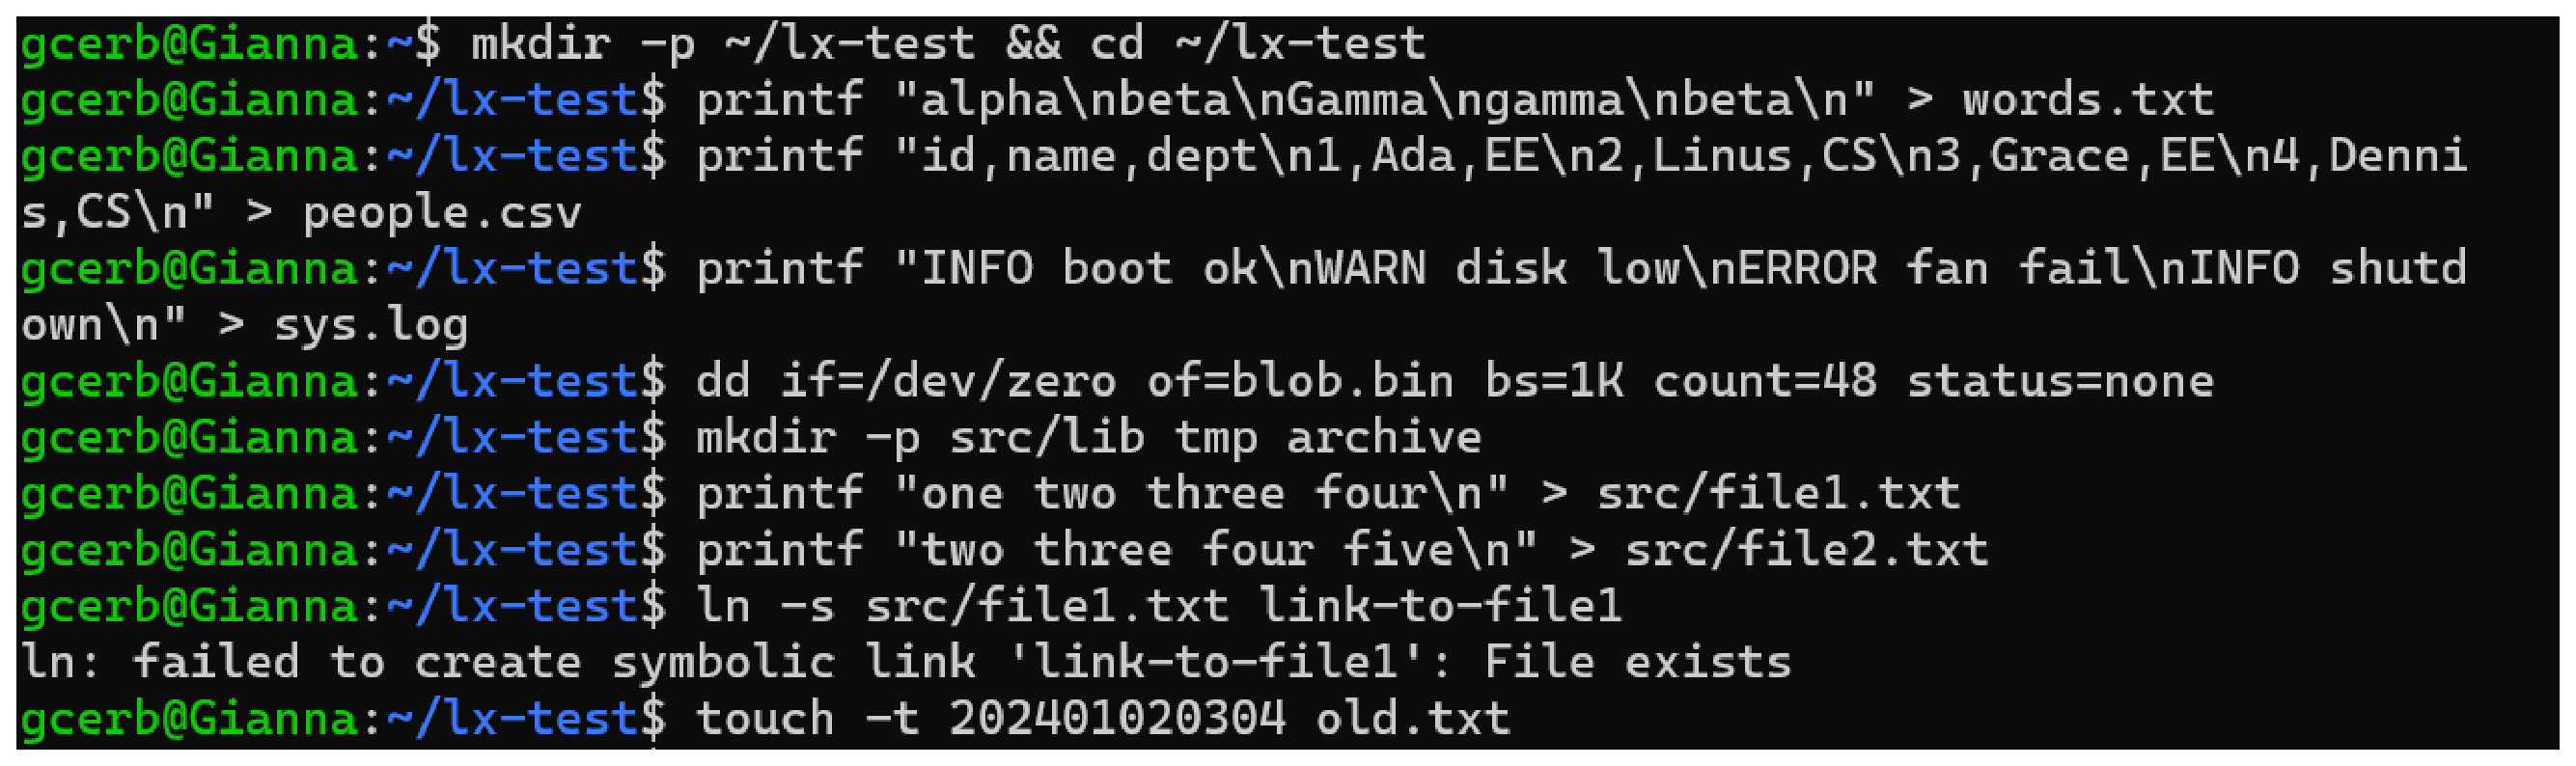
\includegraphics[width=1.0\textwidth]{eps/LinuxBash.eps}
    \caption{Screenshot of Linux Bash commands executed.}
    \label{fig:LinuxBash}
\end{figure}

\section{Linux Problem Set}

\subsection*{A) Navigation \& File Ops}
\begin{verbatim}
1.  pwd
2.  ls -A1
3.  [ -d tmp ] && cp -v src/file1.txt tmp/
4.  mv -v --preserve=timestamps old.txt archive/
5.  touch notes.md  (only if not exists: test -e notes.md || 
(continued) touch notes.md)
6.  du -sh src
\end{verbatim}

\subsection*{B) Viewing \& Searching}
\begin{verbatim}
7.  nl sys.log
8.  grep 'ERROR' sys.log
9.  tr '[:upper:]' '[:lower:]' < words.txt | tr -c '[:alnum:]' '[\n*]' | 
(continued) sort -u | wc -l
10. grep -i '^g' words.txt
11. head -n 2 people.csv
12. tail -n 3 -f sys.log
\end{verbatim}

\subsection*{C) Text Processing}
\begin{verbatim}
13. cut -d',' -f2 people.csv | tail -n +2
14. sort -f words.txt | uniq
15. sed -i.bak 's/three/3/g' src/*
16. wc src/*.txt
\end{verbatim}

\subsection*{D) Permissions \& Ownership}
\begin{verbatim}
17. chmod 700 tmp/
18. chmod -R g+x src/lib
19. stat -c "%a" src/file2.txt
20. chattr +a notes.md
\end{verbatim}

\subsection*{E) Links \& Find}
\begin{verbatim}
21. test -L link-to-file1 && readlink -f link-to-file1
22. find . -type f -size +40k
23. find tmp/ -type f -mmin -10 -exec ls -lh {} +
\end{verbatim}

\subsection*{F) Processes \& Job Control}
\begin{verbatim}
24. pstree -p
25. sleep 120 & echo $!
26. pkill -TERM -u "$USER" sleep
27. ps -eo pid,comm,%mem --sort=-%mem | head -n 6
\end{verbatim}

\subsection*{G) Archiving \& Compression}
\begin{verbatim}
28. tar -czf src.tgz src/
29. tar -tzf src.tgz
30. tar -xzf src.tgz -C tmp src/file2.txt
\end{verbatim}

\subsection*{H) Networking \& System Info}
\begin{verbatim}
31. ss -ltnp
32. ip route show default
33. uname -srm
34. last -n 5
\end{verbatim}

\subsection*{I) Package \& Services (Debian/Ubuntu)}
\begin{verbatim}
35. dpkg -s coreutils | grep Version
36. apt-cache search ripgrep
37. systemctl is-active cron
\end{verbatim}

\subsection*{J) Bash \& Scripting}
\begin{verbatim}
38. for f in src/*.txt; do echo "$f: $(cat "$f")"; done
39. awk -F',' '$3=="CS" && NR>1 {print > "cs.txt"}' people.csv
40. export X=42; echo $X; unset X
\end{verbatim}







\chapter{Project Proposal \\
\small{\textit{-- Justin Baumann, Gianna Cerbone, Thomas Ung, Spurthi Setty}} 
\index{Chapter!ProjectProposal}
\index{ProjectProposal}
\label{Chapter::ProjectProposal}}

% Add a section and label it so that we can reference it later
\section{Project Proposal \label{Section:Description}}

\subsection{Project Title: QuackOps User Interface}

The QuackOps Senior Design project has the following mission statement: 
To develop an autonomous drone delivery system that uses AI for navigation and visual target recognition, and to provide fast, contactless, and efficient on-campus delivery of goods and food.

To aid in the QuackOps Senior Design project, our team will help in developing the graphic user interface with computer vision, AI, and real time updating components from the data gathered by the QuackOps drone. Our contribution will be the web based dashboard that allows users to define delivery parameters, track the drone's location in real time, manage geofences, and monitor fleet health and compliance logs. Our main focus will be the software and user centered interface using DevOps techniques and skills learned in class. 

We will be using Jira KANBAN for task tracking and distribution. Github for source control. CI/CD Actions within GitHub is what we are considering for testing as it is implemented directly into GitHub. Our team needs to make sure that the interface is modular and can be integrated with whatever we are using to get the drone data and can also be able to communicate with the drone in some way. For this part - we will need to think about the drone project extensively and keep both projects intertwined. 


\chapter{AWS Deployment \\
\small{\textit{-- Justin Baumann, Gianna Cerbone, Thomas Ung, Spurthi Setty}} 
\index{Chapter!AWSDeployment}
\index{AWSDeployment}
\label{Chapter::AWS Development}}

\section{Overview}
These instructions are for a Windows machine, assuming Docker and AWS CLI are already installed and an AWS account has been created. These are step-by-step instructions to:
\begin{enumerate}
  \item Configure AWS CLI with IAM Identity Center (SSO).
  \item Push a Docker container image to Amazon Elastic Container Registry (ECR).
  \item Deploy the container image to AWS App Runner.
\end{enumerate}

\section{Set up Environment}
\begin{enumerate}
    \item Ensure that Docker Desktop is installed and open the application 
    \item Open command prompt and navigate to the directory which contains the Dockerfile for the color button app. 
    \item Verify installation of AWS CLI by running the following in your command prompt 
    \begin{minted}
        [fontsize=\small,breaklines]{bash}
        aws --version
    \end{minted}
    You should get an output something like 
    \begin{minted}
        [fontsize=\small,breaklines]{bash}
        aws-cli/2.15.54 Python/3.11.8 Windows/10 exe/AMD64
    \end{minted}
    
\end{enumerate}

\section{Set up IAM Identity Center}
\begin{enumerate}
    \item Login into you AWS Console 
    \item Navigate to IAM Identity Center, and click enable 
    \item On the left hand menu, click on Users and then the Add User button on the top right
    \item Enter the specified username, email and Name. I created a user with the following information 
    \begin{itemize}
        \item username: spurthi
        \item email: spurthi.setty@gmail.com
        \item Display name: Spurthi Setty 
    \end{itemize}
    \item Click on next - no need to fill out additional information or add the user to a group
    \item Select your preferred method of creating a password, I used a one time code, and set up 2FA with my Microsoft authenticator app. 
    \item Follow instructions to verify your email for your user
    \item In your user, click on the tab for AWS Accounts, and then the button called Assign Accounts
    \item Click on Create permissions set $\rightarrow$  predefined $\rightarrow$ Administrator Access 
    \item Assign the access for your user and wait for the confirmation message
    \item Go back to AWS $\rightarrow$ IAM Identity Center $\rightarrow$ Settings. Here you should see a AWS access portal URL. This is your SSO Start URL for the next section. For me it was 
\begin{minted}[fontsize=\small,breaklines]{bash}
https://d-906629391d.awsapps.com/start
\end{minted}
\end{enumerate}



\section{Configure AWS CLI with SSO}
\begin{enumerate}
    \item Run the following command 
\begin{minted}[fontsize=\small,breaklines]{bash}
aws sso login
\end{minted}
    \item You will be prompted to enter a series of inputs, here are the values to provide
    \begin{itemize}
      \item SSO session name: my-sso (or any name)
      \item SSO start URL: https://d-906629391d.awsapps.com/start (or whatever you AWS Access portal URL is)
      \item SSO region: us-east-1
      \item SSO registration scopes: (blank)
    \end{itemize}
    \item The browser will open the url, and the command prompt will aslo provide the URL to an SSO authorization page. 
    \item Enter the username and password on the page for the user you created in the previous section. 
    \item You will then be asked to input a 6 digit code on your browser from you command prompt, or asked to confirm the code.
    \item Approve any permissions and you should get a confirmation message that your request has been approved. 
    \item  You can now close this tab from your browser 
    \item Confirm you have sucessfull logged in by running the following command 
    \begin{minted}[fontsize=\small,breaklines]{base}
        aws sts get-caller-identity
    \end{minted}
    \item Ensure that you are logged in as the user you created with admistrator access. If you are not, then try the sso command again. An example of the expected output for the previous step is
    \begin{minted}[fontsize=\small,breaklines]{json}
    {
    "UserId": "AROAW4ZMTTNJFUQ2BGYAX:spurthi",
    "Account": "474150574930",
    "Arn": "arn:aws:sts::474150574930:assumed-role/AWSReservedSSO_AdministratorAccess_67ee4a10fe53d47e/spurthi"
    }
    \end{minted}
\end{enumerate}


\section{Set Environment Variables (Windows CMD)}

Run the following commands, adjusting names and values are needed. the AWS\_ACCOUNT\_ID should correspond to the value for account in the previous step. The CONTAINER\_PORT should correspond to whatever port is specified in you Dockerfile.
\begin{minted}[fontsize=\small,breaklines]{bat}
set AWS_REGION=us-east-1
set AWS_ACCOUNT_ID=474150574930
set ECR_REPO=color-buttons-app
set IMAGE_TAG=v1
set CONTAINER_PORT=3000
set APP_NAME=my-apprunner-app
\end{minted}

\section{Create an ECR repository}
\begin{enumerate}
    \item Run the following command to describe and create an ECR repository 
    \begin{minted}[fontsize=\small,breaklines]{bat}
    aws ecr describe-repositories --repository-names %ECR_REPO% --region %AWS_REGION% >NUL 2>&1 || ^
    aws ecr create-repository --repository-name %ECR_REPO% --image-scanning-configuration scanOnPush=true --region %AWS_REGION%
    \end{minted}
    \item The output should look something like this\begin{minted}[fontsize=\small,breaklines]{json}
    {
        "repository": {
            "repositoryArn": "arn:aws:ecr:us-east-1:474150574930:repository/color-buttons-app",
            "registryId": "474150574930",
            "repositoryName": "color-buttons-app",
            "repositoryUri": "474150574930.dkr.ecr.us-east-1.amazonaws.com/color-buttons-app",
            "createdAt": "2025-09-29T21:43:04.517000-04:00",
            "imageTagMutability": "MUTABLE",
            "imageScanningConfiguration": {
                "scanOnPush": true
            },
            "encryptionConfiguration": {
                "encryptionType": "AES256"
            }
        }
    }
    \end{minted}
    \item Confirm that the ECR was created by checking it on your AWS console under Elastic Container Registry

\end{enumerate}



\section{Build, Tag, and Push Docker Image}
\begin{enumerate}
    \item Login to docker by running the following command
    \begin{minted}[fontsize=\small,breaklines]{bat}
    aws ecr get-login-password --region %AWS_REGION% | docker login --username AWS --password-stdin %AWS_ACCOUNT_ID%.dkr.ecr.%AWS_REGION%.amazonaws.com
    \end{minted}
    You should get a message that Login succeeded

    \item Build you Docker container by running the following command
    \begin{minted}[fontsize=\small,breaklines]{bat}
    docker build --platform linux/amd64 -t %ECR_REPO%:%IMAGE_TAG% .
    \end{minted}
    If successfull, you terminal should look something like 
    \begin{minted}[fontsize=\small,breaklines]{text}
[+] Building 1.3s (10/10) FINISHED            docker:desktop-linux
\end{minted}

    \item Tag it to your ECR by running the following command
    \begin{minted}[fontsize=\small,breaklines]{bat}
    docker tag %ECR_REPO%:%IMAGE_TAG% %AWS_ACCOUNT_ID%.dkr.ecr.%AWS_REGION%.amazonaws.com/%ECR_REPO%:%IMAGE_TAG%
    \end{minted}

    \item Push your docker container by running the following command 
    \begin{minted}[fontsize=\small,breaklines]{bat}
    docker push %AWS_ACCOUNT_ID%.dkr.ecr.%AWS_REGION%.amazonaws.com/%ECR_REPO%:%IMAGE_TAG%%
    \end{minted}
    If sucessfull, you should see these Images populate in your AWS console within this ECR

    \item Very that the image is pushed by running the following command 
    \begin{minted}[fontsize=\small,breaklines]{bat}
    aws ecr describe-images --repository-name %ECR_REPO% --region %AWS_REGION% --query "imageDetails[].imageTags"
    \end{minted}

    The output should look like this, with whatever you specified the image tag as: 
    \begin{minted}[fontsize=\small,breaklines]{json}
        [
            [
                "v1"
            ]
        ]
        \end{minted}

    
    
    
\end{enumerate}
\section{Create App Runner ECR Access Role}
\begin{enumerate}
  \item Create the role:
\begin{minted}[fontsize=\small,breaklines]{bat}
aws iam create-role --role-name AppRunnerECRAccessRole --assume-role-policy-document "{\"Version\":\"2012-10-17\",\"Statement\":[{\"Effect\":\"Allow\",\"Principal\":{\"Service\":\"build.apprunner.amazonaws.com\"},\"Action\":\"sts:AssumeRole\"}]}"
\end{minted}

  \item Attach the policy:
\begin{minted}[fontsize=\small,breaklines]{bat}
aws iam attach-role-policy --role-name AppRunnerECRAccessRole --policy-arn arn:aws:iam::aws:policy/service-role/AWSAppRunnerServicePolicyForECRAccess
\end{minted}

  \item Save the role ARN in an environment variable:
\begin{minted}[fontsize=\small,breaklines]{bat}
set ACCESS_ROLE_ARN=arn:aws:iam::%AWS_ACCOUNT_ID%:role/AppRunnerECRAccessRole
\end{minted}
\end{enumerate}

\section{Deploy with App Runner}
\begin{enumerate}
  \item Create the App Runner service:
\begin{minted}[fontsize=\small,breaklines]{bat}
aws apprunner create-service ^
--service-name %APP_NAME% ^
--region %AWS_REGION% --profile default ^
--source-configuration "{\"AuthenticationConfiguration\":{\"AccessRoleArn\":\"%ACCESS_ROLE_ARN%\"},\"ImageRepository\":{\"ImageIdentifier\":\"%AWS_ACCOUNT_ID%.dkr.ecr.%AWS_REGION%.amazonaws.com/%ECR_REPO%:%IMAGE_TAG%\",\"ImageRepositoryType\":\"ECR\",\"ImageConfiguration\":{\"Port\":\"%CONTAINER_PORT%\"}},\"AutoDeploymentsEnabled\":true}" ^
--instance-configuration "{\"Cpu\":\"1 vCPU\",\"Memory\":\"2 GB\"}"
\end{minted}
\end{enumerate}

\section{Verify Service and Get URL}
\begin{enumerate}
  \item Check the service status and retrieve the URL:
\begin{minted}[fontsize=\small,breaklines]{bat}
aws apprunner list-services --region %AWS_REGION% --profile default ^
--query "ServiceSummaryList[?ServiceName=='%APP_NAME%'].[ServiceArn,Status,ServiceUrl]" ^
--output table
\end{minted}

\item You can also get the URL by going to AWS App Runner in your console, and clicking the url in the default domain. Here is the App Runner service URL for when I set it up:

\begin{minted}[fontsize=\small]{text}
https://8fjyjsrizv.us-east-1.awsapprunner.com/
\end{minted}

\noindent
You can also access it here: \href{https://8fjyjsrizv.us-east-1.awsapprunner.com/}{https://8fjyjsrizv.us-east-1.awsapprunner.com/}

\end{enumerate}

\section{Website Refactor}

To improve maintainability and follow object-oriented design principles, 
we refactored the JavaScript for the two-buttons application into a class-based design.
The \texttt{ColorController} class encapsulates all button logic.

\subsection{Updated JavaScript Code}

\begin{minted}[fontsize=\small,breaklines]{javascript}
class ColorController {
  constructor(blueBtnId, redBtnId) {
    this.blueBtn = document.getElementById(blueBtnId);
    this.redBtn = document.getElementById(redBtnId);
    this.attachEvents();
  }

  attachEvents() {
    this.blueBtn.addEventListener('click', () => this.setBlue());
    this.redBtn.addEventListener('click', () => this.setRed());
  }

  setBlue() {
    document.body.style.backgroundColor = 'blue';
  }

  setRed() {
    document.body.style.backgroundColor = 'red';
  }
}

document.addEventListener('DOMContentLoaded', () => {
  new ColorController('blueBtn', 'redBtn');
});
\end{minted}

\subsection{UML Class Diagram}

The UML diagram in Figure~\ref{fig:uml-colorcontroller} illustrates the structure of the 
\texttt{ColorController} class.

\begin{figure}[h]
  \centering
  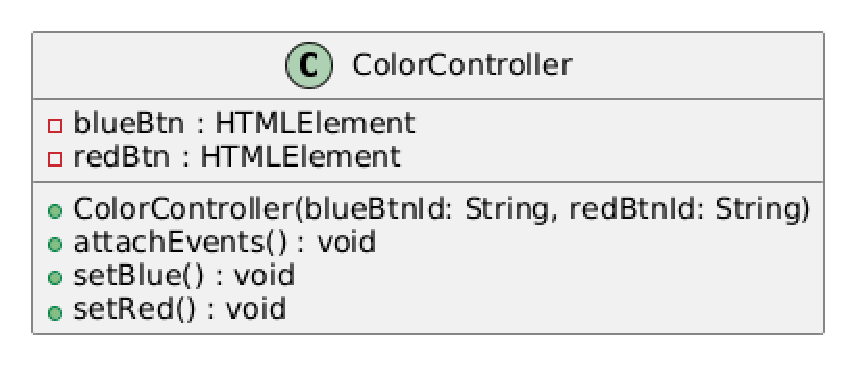
\includegraphics[width=0.6\linewidth]{eps/ColorControllerUML.eps}
  \caption{UML Class Diagram for the \texttt{ColorController} class}
  \label{fig:uml-colorcontroller}
\end{figure}

\chapter{LaTeX Docker \\
\small{\textit{-- Justin Baumann, Gianna Cerbone, Thomas Ung, Spurthi Setty}} 
\index{Chapter!LaTeXDocker}
\index{LaTeXDocker}
\label{Chapter::LaTeXDocker}}

\section{Overview}
This chapter demonstrates building a Docker container that compiles LaTeX documents with TeX Live, similar to how Overleaf runs builds.

\section{Dockerfile}
\begin{minted}[fontsize=\small,breaklines]{docker}
FROM ubuntu:22.04
RUN apt-get update && apt-get install -y \
    texlive-latex-recommended texlive-latex-extra \
    texlive-fonts-recommended latexmk python3-pip \
    && rm -rf /var/lib/apt/lists/*
RUN pip install pygments
WORKDIR /work
ENTRYPOINT ["latexmk","-pdf","-interaction=nonstopmode","-halt-on-error","-shell-escape"]
\end{minted}

\section{Build and Run}
\begin{minted}[fontsize=\small,breaklines]{bash}
# build the image
docker build -t latex-texlive .

# run to compile example.tex into a PDF
docker run --rm -v %cd%:/work latex-texlive example.tex
\end{minted}

\chapter{Bugzilla \\
\small{\textit{-- Spurthi Setty}}
\index{bugzilla} 
\index{Chapter!Bugzilla}
\label{Chapter::Bugzilla}}

\section{Setting Up Bugzilla in Docker on DigitalOcean}

This section documents the detailed procedure for setting up Bugzilla using Docker on a DigitalOcean Ubuntu 22.04 Droplet.  
The setup uses Docker Compose with two services: a MariaDB database and an Apache-based Bugzilla application container.

\subsection{Environment Setup}

\begin{enumerate}
    \item \textbf{Create the Droplet:}  
    - OS: Ubuntu 22.04 LTS  
    - Size: 2 vCPUs, 4 GB RAM (recommended minimum)  
    - Note the public IP address (e.g., \texttt{167.99.54.162}).

    \item \textbf{Update and Install Docker:}

    \begin{minted}[fontsize=\small,breaklines]{bash}
sudo apt update && sudo apt upgrade -y
sudo apt install docker.io docker-compose -y
sudo systemctl enable docker
sudo systemctl start docker
docker --version
docker compose version
    \end{minted}

    \item \textbf{Verify Docker Installation:}

    \begin{minted}[fontsize=\small,breaklines]{bash}
docker --version
docker compose version
    \end{minted}
\end{enumerate}

\subsection{Deploying Bugzilla via Docker Compose}

\begin{enumerate}
    \item \textbf{Create Directory Structure:}

    \begin{minted}[fontsize=\small,breaklines]{bash}
mkdir -p /opt/bugzilla
cd /opt/bugzilla
    \end{minted}

    \item \textbf{Create the Docker Compose File:}

    \begin{minted}[fontsize=\small,breaklines]{yaml}
version: '3'
services:
  db:
    image: mariadb:10.6
    restart: always
    environment:
      MYSQL_ROOT_PASSWORD: root
      MYSQL_DATABASE: bugzilla
      MYSQL_USER: bugs
      MYSQL_PASSWORD: bugs
    volumes:
      - bugzilla_db_data:/var/lib/mysql

  bugzilla:
    image: bugzilla/bugzilla-dev:latest
    restart: always
    ports:
      - "8080:80"
    depends_on:
      - db
    volumes:
      - bugzilla_data:/var/www/html/bugzilla

volumes:
  bugzilla_db_data:
  bugzilla_data:
    \end{minted}

    \item \textbf{Start the Containers:}

    \begin{minted}[fontsize=\small,breaklines]{bash}
docker compose up -d
docker ps
    \end{minted}

    The Bugzilla service listens on port \texttt{8080} on the host, mapped to port \texttt{80} inside the container.
\end{enumerate}

\subsection{Configuring Bugzilla Inside the Container}

\begin{enumerate}
    \item \textbf{Access the Running Container:}

    \begin{minted}[fontsize=\small,breaklines]{bash}
docker exec -it bugzilla-bugzilla-1 bash
    \end{minted}

    \item \textbf{Create and Configure the Database:}

    \begin{minted}[fontsize=\small,breaklines]{bash}
mysql -uroot -e "CREATE DATABASE IF NOT EXISTS bugzilla CHARACTER SET utf8mb4;"
mysql -uroot -e "CREATE USER 'bugs'@'localhost' IDENTIFIED BY 'bugs';"
mysql -uroot -e "GRANT ALL PRIVILEGES ON bugzilla.* TO 'bugs'@'localhost'; FLUSH PRIVILEGES;"
    \end{minted}

    \item \textbf{Set Up Bugzilla Configuration:}

    \begin{minted}[fontsize=\small,breaklines]{bash}
cd /var/www/html/bugzilla
cat > localconfig <<'CONF'
$db_driver = 'mysql';
$db_host   = 'localhost';
$db_name   = 'bugzilla';
$db_user   = 'bugs';
$db_pass   = 'bugs';
$webservergroup = 'apache';
$urlbase = 'http://167.99.54.162:8080/bugzilla/';
CONF
chown -R apache:apache .
    \end{minted}

    \item \textbf{Initialize Bugzilla:}

    \begin{minted}[fontsize=\small,breaklines]{bash}
perl checksetup.pl
    \end{minted}

    The script validates Perl modules, initializes the database schema, and generates the \texttt{params.json} configuration file.
\end{enumerate}

\subsection{Resolving Apache Configuration and Permissions}

\begin{enumerate}
    \item \textbf{Fix Permissions:}

    \begin{minted}[fontsize=\small,breaklines]{bash}
chown -R apache:apache /var/www/html/bugzilla
chmod -R 755 /var/www/html/bugzilla
    \end{minted}

    \item \textbf{Replace the Default Apache Configuration:}

    \begin{minted}[fontsize=\small,breaklines]{bash}
rm -f /etc/httpd/conf.d/welcome.conf
cat >/etc/httpd/conf.d/bugzilla-root.conf <<'CONF'
ServerName 127.0.0.1
DocumentRoot "/var/www/html/bugzilla"

<Directory "/var/www/html/bugzilla">
    Options +ExecCGI +FollowSymLinks
    AllowOverride All
    Require all granted
    AddHandler cgi-script .cgi
</Directory>

DirectoryIndex index.cgi
CONF
    \end{minted}

    \item \textbf{Restart Apache (no systemd available):}

    \begin{minted}[fontsize=\small,breaklines]{bash}
pkill -f httpd || true
/usr/sbin/httpd -DFOREGROUND &
    \end{minted}
\end{enumerate}

\subsection{Testing and Verification}

\begin{enumerate}
    \item \textbf{Verify Local Connectivity:}

    \begin{minted}[fontsize=\small,breaklines]{bash}
curl -I http://127.0.0.1/bugzilla/
    \end{minted}

    Expect either \texttt{HTTP/1.1 200 OK} or \texttt{302 Found (index.cgi)}.

    \item \textbf{Verify Host Mapping:}

    \begin{minted}[fontsize=\small,breaklines]{bash}
curl -I http://127.0.0.1:8080/
    \end{minted}

    \item \textbf{Access the Web Interface:}

    \begin{minted}[fontsize=\small,breaklines]{bash}
http://167.99.54.162:8080/
    \end{minted}

    Log in with:
    \begin{verbatim}
    admin@example.com / admin123
    \end{verbatim}
\end{enumerate}

\subsection{Troubleshooting Notes}

\begin{itemize}
    \item \textbf{403 Forbidden Error:}  
    Fixed by defining explicit \texttt{Require all granted} and enabling CGI execution in Apache config.

    \item \textbf{500 Internal Server Error:}  
    Caused by missing \texttt{params.json}; running \texttt{perl checksetup.pl} regenerates it.

    \item \textbf{Apache Startup Errors:}  
    If logs are missing, recreate them:
    \begin{minted}[fontsize=\small,breaklines]{bash}
mkdir -p /var/log/httpd
touch /var/log/httpd/error_log /var/log/httpd/access_log
chown -R apache:apache /var/log/httpd
    \end{minted}

    \item \textbf{Testing Without Browser:}  
    Use:
    \begin{minted}[fontsize=\small,breaklines]{bash}
curl -I http://127.0.0.1/bugzilla/
    \end{minted}
\end{itemize}

\subsection{Final Result}

Bugzilla was successfully deployed and is accessible at:

\begin{center}
\textbf{\url{http://167.99.54.162:8080/}}
\end{center}
\begin{figure}
    \centering
    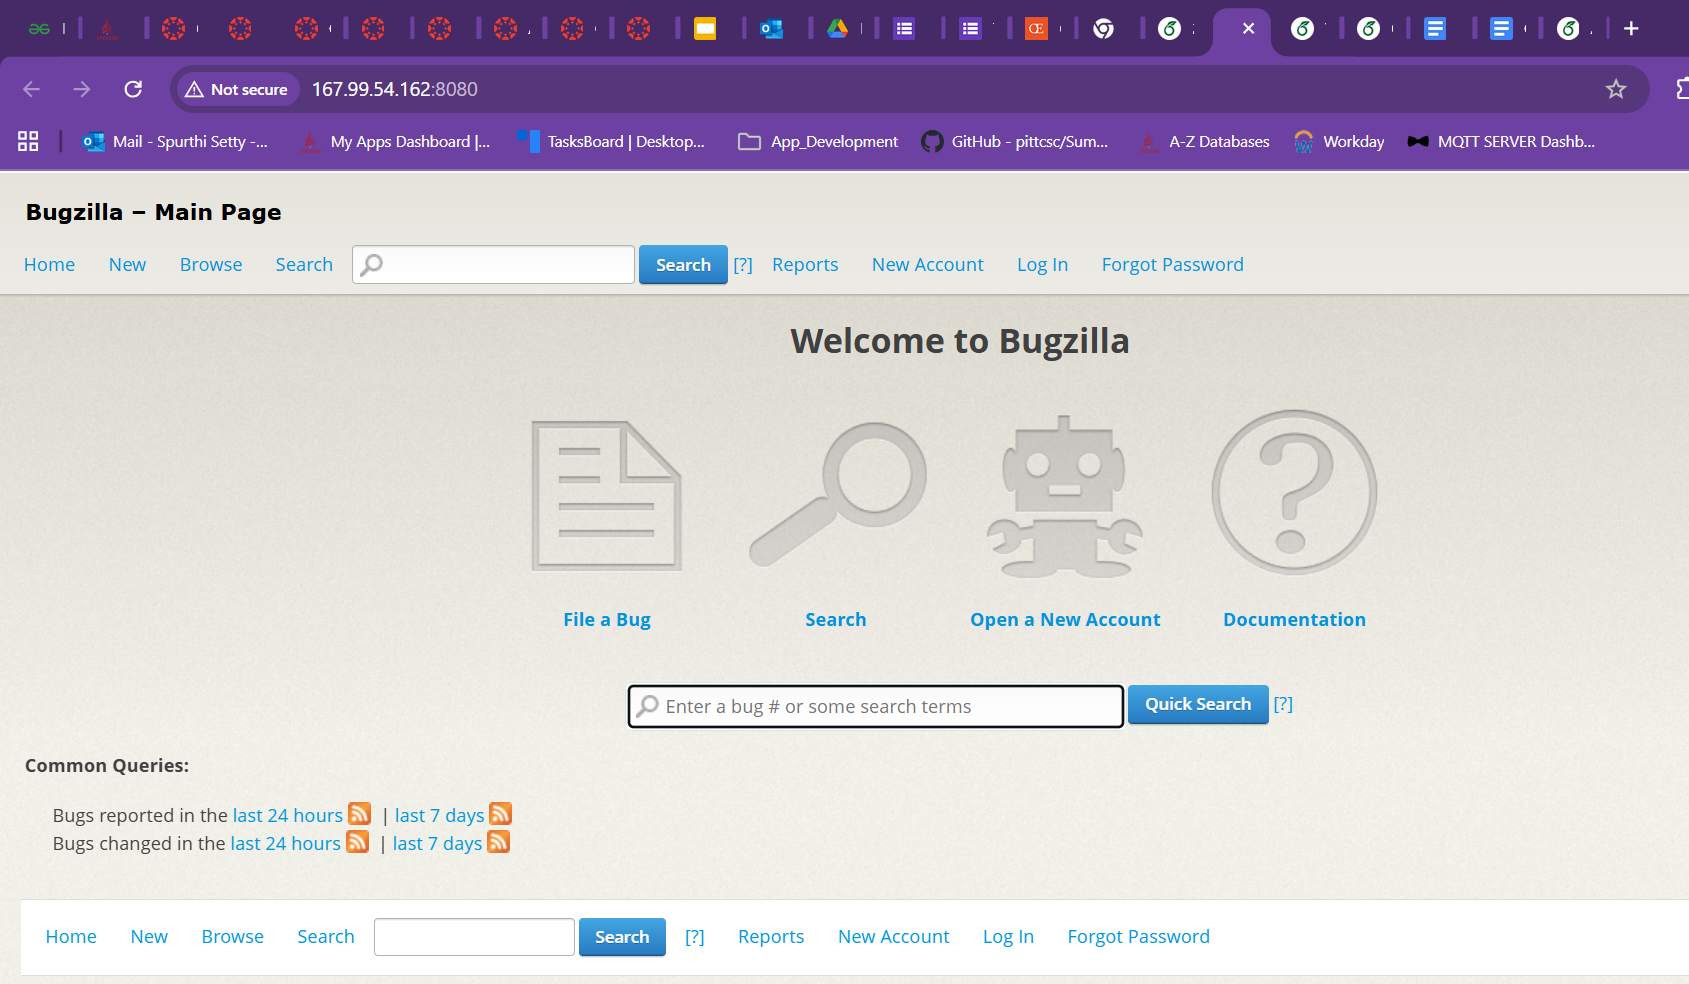
\includegraphics[width=0.7\linewidth]{png/bugzilla.png}
    \caption{Screenshot of bugzilla working at \url{http://167.99.54.162:8080/} }
    \label{fig:placeholder}
\end{figure}
This configuration persists through container restarts, with all data stored in Docker volumes defined in the Compose file.

\chapter{Overleaf \\
\small{\textit{-- Spurthi Setty}}
\index{bugzilla} 
\index{Chapter!Overleaf}
\label{Chapter::Overleaf}}

\section{How to compile this chapter}
Add to your preamble and compile with shell-escape to enable \texttt{minted}:
\begin{minted}[fontsize=\small]{latex}
\usepackage{xcolor}
\usepackage{minted}
\setminted{fontsize=\small,breaklines=true}
% Compile with:  latexmk -pdf -shell-escape main.tex
\end{minted}

\section{Context}
We deployed \textbf{Overleaf Community Edition} on an existing DigitalOcean droplet that already served another site on \url{http://167.99.54.162:8080}. To avoid port conflicts, Overleaf was mapped to port \texttt{8090}.

\section{Prerequisites (Ubuntu 22.04/24.04)}
\begin{minted}[fontsize=\small]{bash}
# optional: install Docker Engine + compose plugin (if not present)
apt-get update -y
apt-get install -y ca-certificates curl gnupg lsb-release
install -m 0755 -d /etc/apt/keyrings
curl -fsSL https://download.docker.com/linux/ubuntu/gpg | gpg --dearmor -o /etc/apt/keyrings/docker.gpg
chmod a+r /etc/apt/keyrings/docker.gpg
echo "deb [arch=$(dpkg --print-architecture) signed-by=/etc/apt/keyrings/docker.gpg] \
https://download.docker.com/linux/ubuntu $(lsb_release -cs) stable" \
| tee /etc/apt/sources.list.d/docker.list > /dev/null
apt-get update -y
apt-get install -y docker-ce docker-ce-cli containerd.io docker-buildx-plugin docker-compose-plugin
systemctl enable --now docker

# sanity
docker --version
docker compose version
\end{minted}

\section{Baseline deployment}
\subsection{Create working directory}
\begin{minted}{bash}
mkdir -p /opt/overleaf
cd /opt/overleaf
\end{minted}

\subsection{Open firewall}
\begin{minted}{bash}
ufw allow OpenSSH
ufw allow 8090/tcp
ufw --force enable
ufw status
\end{minted}

\subsection{Initial \texttt{docker-compose.yml}}
We used \texttt{sharelatex/sharelatex} (the Overleaf CE image) with MongoDB and Redis. Note the \textbf{Overleaf-branded} env vars and the \textbf{new data path} \texttt{/var/lib/overleaf}.
\begin{minted}[fontsize=\small]{yaml}
services:
  mongo:
    image: mongo:6.0
    restart: unless-stopped
    volumes:
      - overleaf_mongo_data:/data/db

  redis:
    image: redis:7
    restart: unless-stopped
    command: ["redis-server","--appendonly","yes"]
    volumes:
      - overleaf_redis_data:/data

  sharelatex:
    image: sharelatex/sharelatex:latest
    container_name: sharelatex
    restart: unless-stopped
    depends_on:
      - mongo
      - redis
    environment:
      OVERLEAF_SITE_URL: "http://167.99.54.162:8090"
      OVERLEAF_MONGO_URL: "mongodb://mongo:27017/sharelatex"
      OVERLEAF_REDIS_HOST: "redis"
    ports:
      - "8090:80"
    volumes:
      - overleaf_app_data:/var/lib/overleaf

volumes:
  overleaf_mongo_data:
  overleaf_redis_data:
  overleaf_app_data:
\end{minted}

\subsection{Start the stack}
\begin{minted}{bash}
cd /opt/overleaf
docker compose pull
docker compose up -d
docker compose ps
\end{minted}

\section{Issues encountered and exact fixes}
Below are the exact errors we hit and the precise commands that resolved them on this host.

\subsection{(A) Wrong image / registry hiccup}
\textit{Symptom:} Pull errors for \texttt{ghcr.io/overleaf/overleaf} (access denied/registry auth).\\
\textit{Fix:} Switch to Docker Hub image \texttt{sharelatex/sharelatex}.
\begin{minted}{bash}
# if your compose ever referenced ghcr, replace it with Docker Hub image
sed -i 's#ghcr.io/overleaf/overleaf:latest#sharelatex/sharelatex:latest#' docker-compose.yml
\end{minted}

\subsection{(B) Legacy bind mount path: \texttt{/var/lib/sharelatex}}
\textit{Symptom:} Container logs show rebranding guard refusing to start due to old path.\\
\textit{Fix:} Use the new path \texttt{/var/lib/overleaf} in the bind mount.
\begin{minted}{bash}
sed -i 's#/var/lib/sharelatex#/var/lib/overleaf#g' docker-compose.yml
\end{minted}

\subsection{(C) Legacy env var names: \texttt{SHARELATEX\_*}}
\textit{Symptom:} \texttt{000\_check\_for\_old\_env\_vars\_5.sh} refuses startup, listing \texttt{SHARELATEX\_MONGO\_URL}, \texttt{SHARELATEX\_REDIS\_HOST}, \texttt{SHARELATEX\_SITE\_URL}.\\
\textit{Fix:} Rename to the Overleaf-branded variants.
\begin{minted}{bash}
sed -i -E 's/SHARELATEX_MONGO_URL/OVERLEAF_MONGO_URL/g; \
s/SHARELATEX_REDIS_HOST/OVERLEAF_REDIS_HOST/g; \
s/SHARELATEX_SITE_URL/OVERLEAF_SITE_URL/g' docker-compose.yml

# if you had a .env with legacy keys, update it too
sed -i 's/SHARELATEX_SITE_URL/OVERLEAF_SITE_URL/' .env 2>/dev/null || true
\end{minted}

\subsection{(D) Connection reset / app crash loop due to Mongo transactions}
\textit{Symptom:} Logs show: \texttt{Transaction numbers are only allowed on a replica set member or mongos}.\\
\textit{Cause:} Overleaf 5+ expects MongoDB with transactions support (i.e., a replica set), even for a single node.\\
\textit{Fix:} Run Mongo as a single-node replica set and update the connection string.

\paragraph{Step D1: Add override to enable replica set and connection string}
\begin{minted}{bash}
cat > docker-compose.override.yml <<'YML'
services:
  mongo:
    command: ["mongod","--replSet","rs0","--bind_ip_all"]
  sharelatex:
    environment:
      OVERLEAF_MONGO_URL: "mongodb://mongo:27017/sharelatex?replicaSet=rs0"
YML
\end{minted}

\paragraph{Step D2: Recreate the stack}
\begin{minted}{bash}
docker compose down
docker compose up -d
\end{minted}

\paragraph{Step D3: Initialize the replica set (one-time)}
\begin{minted}{bash}
# try mongosh (6.x); fallback to legacy mongo shell if needed
docker exec overleaf-mongo-1 bash -lc \
  'mongosh --quiet --eval "rs.initiate({_id:\"rs0\", members:[{_id:0, host:\"mongo:27017\"}]})"' \
  || docker exec overleaf-mongo-1 bash -lc \
  'mongo --quiet --eval "rs.initiate({_id:\"rs0\", members:[{_id:0, host:\"mongo:27017\"}]})"'
\end{minted}

\paragraph{Step D4: Verify replica set is healthy}
\begin{minted}{bash}
docker exec overleaf-mongo-1 bash -lc 'mongosh --quiet --eval "rs.status().ok"' \
  || docker exec overleaf-mongo-1 bash -lc 'mongo --quiet --eval "rs.status().ok"'
# expect: 1
\end{minted}

\subsection{(E) Optional: tune kernel warning from Redis}
\begin{minted}{bash}
# not required for functionality, but silences Redis warning
sysctl -w vm.overcommit_memory=1
echo 'vm.overcommit_memory=1' >> /etc/sysctl.conf
\end{minted}

\section{Verification commands we used}
\begin{minted}{bash}
# container status
cd /opt/overleaf
docker compose ps

# app health (host)
curl -I http://localhost:8090
curl -sS http://localhost:8090/health_check || true

# service status inside the container (runit + port 80)
docker exec -it sharelatex bash -lc 'sv status nginx; sv status sharelatex; ss -tlnp | grep :80 || true'

# logs (when diagnosing)
docker compose logs --tail=200 sharelatex
\end{minted}

\section{Accessing the site}
First-time admin setup (\textit{Launchpad}):
\url{http://167.99.54.162:8090/launchpad}
After creating the admin, use the main URL:
\url{http://167.99.54.162:8090}

\section{Maintenance cheatsheet}
\begin{minted}{bash}
# restart
cd /opt/overleaf
docker compose down
docker compose up -d

# upgrade images (occasional)
docker compose pull && docker compose up -d

# view logs
docker compose logs -f sharelatex

# backups of volumes (quick tar via busybox)
mkdir -p /opt/overleaf/backups
cd /opt/overleaf
for v in overleaf_app_data overleaf_mongo_data overleaf_redis_data; do
  docker run --rm -v ${v}:/data -v $(pwd)/backups:/backup busybox \
    tar czf /backup/${v}_$(date +%F).tar.gz /data
done
\end{minted}

\section{Final status}
After applying fixes (B) path update, (C) env var rename to \texttt{OVERLEAF\_*}, and (D) enabling a single-node Mongo replica set, Overleaf CE started cleanly and became reachable at \url{http://167.99.54.162:8090}. The \texttt{/launchpad} route was used to create the initial admin account.

\begin{figure}
    \centering
    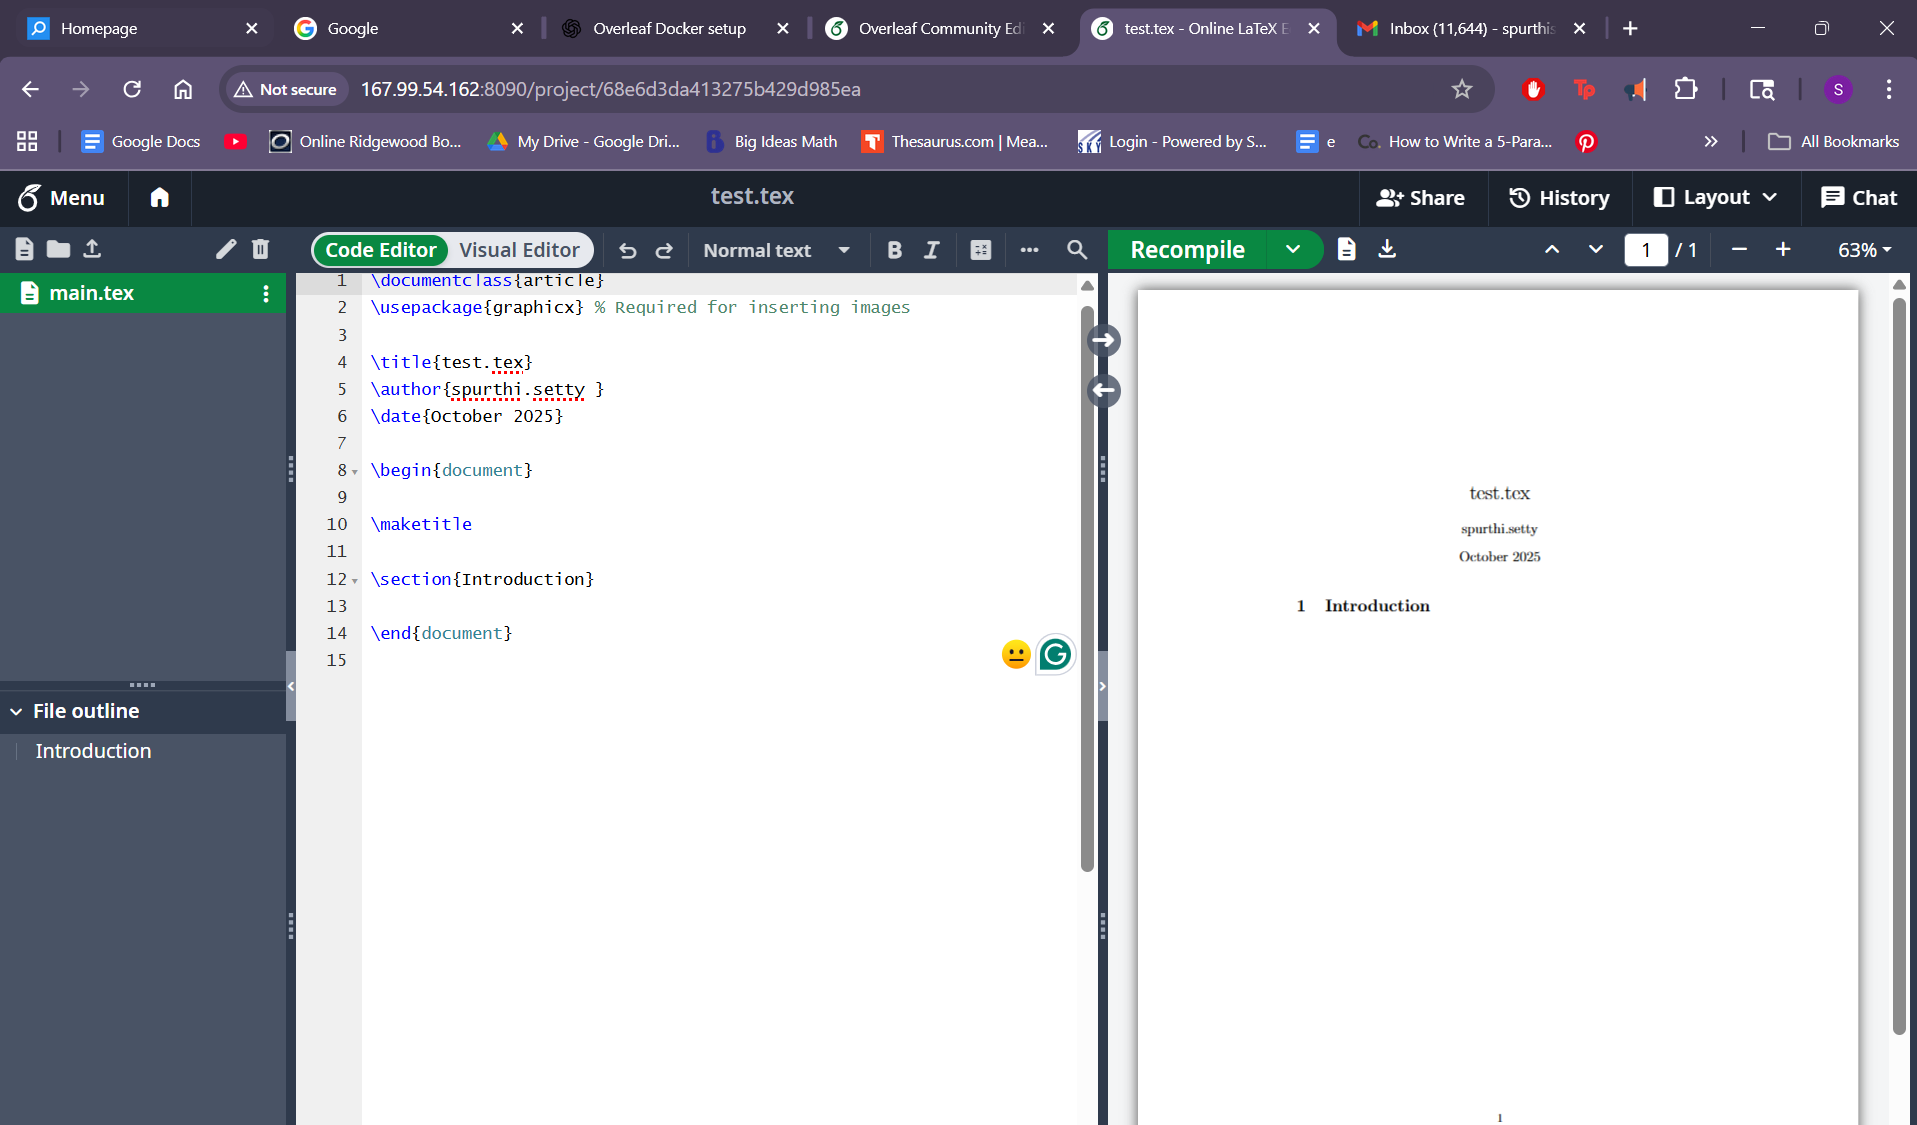
\includegraphics[width=0.9\linewidth]{png/overleaf.png}
    \caption{Screenshot of Compiled File at \url{http://167.99.54.162:8090}}
    \label{fig:placeholder}
\end{figure}


\section{Creating a New User Account}

To create a new account manually from the administrator dashboard, follow these steps:

\begin{enumerate}
  \item \textbf{Login as an administrator.}
        Open your Overleaf instance and sign in with your admin credentials.
  \item \textbf{Open the Manage Users panel.}
        Click on your profile icon at the top right corner and select \texttt{Manage Users}.
  \item \textbf{Register the new user.}
        In the user management form, enter the email address of the new user and click \texttt{Register}.
  \item \textbf{Access the Set Password page.}
        Copy the \texttt{Set Password} URL generated for that user and paste it into your browser.
  \item \textbf{Set a new password.}
        The page will prompt you to create a new password for the account. Enter the desired password and confirm it.
  \item \textbf{Activate and log in.}
        After setting the password, click \texttt{Activate}. The user can now log in using the new credentials.
\end{enumerate}

\chapter{SSL Research}
\small{\textit{-- Gianna Cerbone}}
\label{Chapter:SSLResearch}
\index{Chapter!SSLResearch}

\section{Overview}

This chapter summarizes the research conducted on implementing SSL (Secure Sockets Layer) for Overleaf containers and images. The focus is on how to add SSL certificates, manage them using free services such as Let’s Encrypt, and automate their renewal process. Let’s Encrypt provides free certificates that expire every 90 days, making automated renewal a critical part of the configuration.

\section{Architecture Considerations}

In most deployments, Overleaf is hosted using Docker containers or the Overleaf Toolkit. The recommended approach is to run Overleaf behind a reverse proxy (commonly Nginx) that handles TLS termination. This means HTTPS traffic is decrypted at the proxy, which then forwards plain HTTP requests to the Overleaf application container.

Embedding SSL certificate management directly inside the Overleaf container is possible but discouraged. It adds unnecessary complexity and makes updates harder. Managing certificates at the proxy layer is simpler, more secure, and allows reuse of certificates for multiple services.

\section{Using the Overleaf Toolkit with TLS Proxy Mode}

For those using the Overleaf Toolkit, TLS support is already integrated. You can enable it by initializing the toolkit with:

\begin{verbatim}
bin/init --tls
\end{verbatim}

This generates an Nginx configuration and placeholder certificates located in:
\begin{verbatim}
config/nginx/certs/overleaf_certificate.pem
config/nginx/certs/overleaf_key.pem
\end{verbatim}

Replace these placeholder files with your actual SSL certificate and key. The following settings can be configured in \texttt{config/overleaf.rc}:

\begin{verbatim}
NGINX_ENABLED=true
NGINX_CONFIG_PATH=config/nginx/nginx.conf
NGINX_HTTP_PORT=80
TLS_CERTIFICATE_PATH=config/nginx/certs/overleaf_certificate.pem
TLS_PRIVATE_KEY_PATH=config/nginx/certs/overleaf_key.pem
TLS_PORT=443
\end{verbatim}

After modifying these settings, re-run:
\begin{verbatim}
bin/up
\end{verbatim}
to recreate and restart the containers.

If an external proxy handles SSL termination, add the proxy IP address to:
\begin{verbatim}
OVERLEAF_TRUSTED_PROXY_IPS
\end{verbatim}
so that Overleaf correctly interprets forwarded HTTPS requests.

\section{Using an External Reverse Proxy}

Another common approach is to use an external reverse proxy, such as Nginx or Traefik, to manage SSL and forward traffic to the Overleaf container. This approach simplifies certificate management and keeps the Overleaf image lightweight.

\subsection{Advantages}
\begin{itemize}
    \item TLS configuration is isolated from the Overleaf container.
    \item Certificates can be easily renewed and reused for other services.
    \item Simplifies upgrades to Overleaf since SSL is handled separately.
\end{itemize}

\subsection{Example Nginx Configuration}

\begin{verbatim}
server {
    listen 80;
    server_name overleaf.example.com;

    location /.well-known/acme-challenge/ {
        root /var/www/acme-challenges;
    }

    location / {
        proxy_pass http://127.0.0.1:8000;
        proxy_http_version 1.1;
        proxy_set_header Upgrade $http_upgrade;
        proxy_set_header Connection "upgrade";
        proxy_set_header Host $host;
        proxy_set_header X-Forwarded-Proto $scheme;
        proxy_set_header X-Real-IP $remote_addr;
    }
}

server {
    listen 443 ssl;
    server_name overleaf.example.com;

    ssl_certificate /etc/letsencrypt/live/overleaf.example.com/fullchain.pem;
    ssl_certificate_key /etc/letsencrypt/live/overleaf.example.com/privkey.pem;

    location / {
        proxy_pass http://127.0.0.1:8000;
        proxy_http_version 1.1;
        proxy_set_header Upgrade $http_upgrade;
        proxy_set_header Connection "upgrade";
        proxy_set_header Host $host;
        proxy_set_header X-Forwarded-Proto $scheme;
        proxy_set_header X-Real-IP $remote_addr;
    }
}
\end{verbatim}

\section{Using Let’s Encrypt for Free SSL Certificates}

Let’s Encrypt offers free SSL certificates that are valid for 90 days. To generate and install one using \texttt{certbot}, run the following commands:

\begin{verbatim}
sudo apt install certbot python3-certbot-nginx
sudo certbot certonly --webroot -w /var/www/acme-challenges \
    -d overleaf.example.com
\end{verbatim}

After the certificate is installed, configure automatic renewal:

\begin{verbatim}
sudo certbot renew --post-hook "systemctl reload nginx"
\end{verbatim}

The renewal command can be added to a cron job or systemd timer to run periodically.

\section{Renewal and Automation}

Because Let’s Encrypt certificates expire every three months, it is essential to automate the renewal process. Recommended best practices include:
\begin{itemize}
    \item Schedule automatic renewals using \texttt{certbot renew}.
    \item Reload or restart the Nginx proxy after renewal to apply the new certificate.
    \item Test renewal scripts regularly using the \texttt{--dry-run} flag.
    \item Ensure that HTTP port 80 is available for ACME challenge responses.
\end{itemize}

\section{Installing Certificates Inside the Container (Not Recommended)}

While possible, installing and managing SSL certificates inside the Overleaf container is not recommended. This approach introduces additional maintenance complexity, such as updating trust stores, managing permissions, and triggering restarts on renewal.

If necessary, certificates can be mounted as Docker volumes and renewed via a sidecar container running \texttt{certbot}. The containerized Overleaf application would then reload the updated certificates periodically.

\section{Summary and Recommendations}

\begin{itemize}
    \item Use a reverse proxy such as Nginx to handle SSL termination.
    \item Use Let’s Encrypt for free, automated SSL certificates that renew every 90 days.
    \item In the Overleaf Toolkit, enable TLS with \texttt{bin/init --tls} and replace the default certificates.
    \item If using an external proxy, ensure websockets and headers (\texttt{Upgrade}, \texttt{X-Forwarded-Proto}) are properly forwarded.
    \item Avoid embedding certificate management logic inside the Overleaf application container.
\end{itemize}

By following these practices, Overleaf can be securely deployed with HTTPS, using automated and renewable SSL certificates, ensuring both encrypted communication and reduced administrative overhead.

\chapter{Configuring Overleaf with Full LaTeX Package Support}

\small{\textit{-- Spurthi Setty}}
\label{Chapter:OverleafConfiguration}
\index{Chapter!OverleafConfiguration}

\section{Introduction}

In order to compile LaTeX documents with advanced packages such as \verb|tikz|, \verb|pgfplots|, and \verb|minted|, it is necessary to configure Overleaf's self-hosted Docker environment with the full \TeX{} Live distribution. This chapter outlines the complete setup process, including Docker configuration, LaTeX package installation, troubleshooting missing packages, and environment adjustments to ensure Overleaf compiles documents without errors.

\section{Setting Up Overleaf with Docker}

We used the official \verb|sharelatex/sharelatex| Docker image as a base and extended it with the full \TeX{} Live distribution to ensure comprehensive package support.

\subsection{Directory Structure}

All files were placed under:

\begin{minted}{bash}
/opt/overleaf/
\end{minted}

Key files include:

\begin{itemize}
  \item \texttt{Dockerfile} – to install \texttt{texlive-full}
  \item \texttt{docker-compose.yml} – to define Overleaf, MongoDB, and Redis services
\end{itemize}

\subsection{Dockerfile}

The Dockerfile extends the base image and installs \TeX{} Live:

\begin{minted}{dockerfile}
FROM sharelatex/sharelatex:latest

USER root

RUN apt-get update && \
    apt-get install -y texlive-full && \
    apt-get clean && rm -rf /var/lib/apt/lists/*

ENV TEXMFROOT=/usr/share/texlive
ENV TEXMFVAR=$TEXMFROOT/texmf-var
ENV TEXMFSYSVAR=$TEXMFROOT/texmf-var
ENV TEXMFCONFIG=$TEXMFROOT/texmf-config
ENV TEXMFSYSCONFIG=$TEXMFROOT/texmf-config
ENV TEXMFLOCAL=$TEXMFROOT/texmf-local
ENV TEXMFDIST=$TEXMFROOT/texmf-dist
ENV TEXMFHOME=/root/texmf

RUN mktexlsr
\end{minted}

\subsection{docker-compose.yml}

The Docker Compose configuration links Overleaf with MongoDB and Redis:

\begin{minted}{yaml}
services:
  sharelatex:
    image: overleaf-fulltex
    container_name: sharelatex
    restart: unless-stopped
    ports:
      - "8090:80"
    environment:
      OVERLEAF_SITE_URL: "http://<YOUR_SERVER_IP>:8090"
      OVERLEAF_MONGO_URL: "mongodb://mongo/sharelatex"
      OVERLEAF_REDIS_HOST: "redis"
    volumes:
      - overleaf_app_data:/var/lib/overleaf

  mongo:
    image: mongo:6.0
    container_name: overleaf-mongo-1
    restart: unless-stopped
    volumes:
      - overleaf_mongo_data:/data/db
    command: ["mongod", "--replSet", "rs0", "--bind_ip_all"]

  redis:
    image: redis:7
    container_name: overleaf-redis-1
    restart: unless-stopped
    command: ["redis-server", "--appendonly", "yes"]
    volumes:
      - overleaf_redis_data:/data

volumes:
  overleaf_app_data:
  overleaf_mongo_data:
  overleaf_redis_data:
\end{minted}

\subsection{Enabling MongoDB Replica Set}

Overleaf requires MongoDB to support transactions, which are only available in replica sets. After container startup, we enabled the replica set manually:

\begin{minted}{bash}
docker exec -it overleaf-mongo-1 mongosh
> rs.initiate()
\end{minted}

\subsection{Building and Starting Containers}

After creating the Dockerfile and docker-compose.yml, we built the custom image:

\begin{minted}{bash}
cd /opt/overleaf
docker build -t overleaf-fulltex .
\end{minted}

Then started all services:

\begin{minted}{bash}
docker-compose up -d
\end{minted}

\subsection{Verifying Initial Package Availability}

After building and starting the containers, we confirmed that LaTeX packages such as \verb|tikz|, \verb|pgfplots|, and \verb|psfrag| were available by executing:

\begin{minted}{bash}
docker exec -it sharelatex kpsewhich tikz.sty
docker exec -it sharelatex kpsewhich pgfplots.sty
docker exec -it sharelatex kpsewhich psfrag.sty
\end{minted}

If no path was returned, we updated the environment variables inside the container to point to the correct \TeX{} Live installation path and rebuilt the file name database with:

\begin{minted}{bash}
docker exec -it sharelatex mktexlsr
\end{minted}

\section{Troubleshooting Missing LaTeX Packages}

After successfully deploying Overleaf with the full \TeX{} Live distribution, we encountered several missing package errors when attempting to compile a Cornell University thesis template. This section documents the systematic troubleshooting process used to identify and install missing LaTeX packages.

\subsection{Initial Environment Configuration}

Our Overleaf deployment consisted of three Docker containers running on an Ubuntu virtual machine hosted on Digital Ocean:

\begin{itemize}
  \item \texttt{sharelatex} – Overleaf application server (image: \texttt{overleaf-fulltex})
  \item \texttt{overleaf-mongo-1} – MongoDB 6.0 database
  \item \texttt{overleaf-redis-1} – Redis 7 cache server
\end{itemize}

The containers were accessible via port 8090 on the host machine at \texttt{http://167.99.54.162:8090}, running \TeX{} Live 2025.

\subsection{Verifying Container Status}

Before beginning troubleshooting, we verified that all containers were running properly:

\begin{minted}{bash}
docker ps
\end{minted}

Expected output:

\begin{minted}{text}
CONTAINER ID   IMAGE              COMMAND           CREATED      STATUS      PORTS                    NAMES
7244bdc99c8a   overleaf-fulltex   "/sbin/my_init"   2 hours ago  Up 2 hours  0.0.0.0:8090->80/tcp     sharelatex
9b8786881b61   redis:7            "docker-entry..."  2 hours ago  Up 2 hours  6379/tcp                 overleaf-redis-1
3f1ee20cf169   mongo:6.0          "docker-entry..."  2 hours ago  Up 2 hours  27017/tcp                overleaf-mongo-1
\end{minted}

\subsection{Sequential Package Installation}

\subsubsection{Missing Package: \texttt{psfrag}}

The first compilation error indicated a missing \verb|psfrag.sty| file:

\begin{minted}{text}
! LaTeX Error: File `psfrag.sty' not found.

Type X to quit or <RETURN> to proceed,
or enter new name. (Default extension: sty)

Enter file name: 
! Emergency stop.
\end{minted}

We verified whether the package was already installed:

\begin{minted}{bash}
docker exec -it sharelatex tlmgr info psfrag
\end{minted}

The output confirmed the package was installed, but the \TeX{} filename database needed updating:

\begin{minted}{bash}
docker exec -it sharelatex mktexlsr
\end{minted}

We verified the package file location:

\begin{minted}{bash}
docker exec -it sharelatex find /usr/local/texlive -name "psfrag.sty"
\end{minted}

Result: \texttt{/usr/local/texlive/2025/texmf-dist/tex/latex/psfrag/psfrag.sty}

Finally, we restarted the container:

\begin{minted}{bash}
docker restart sharelatex
\end{minted}

\subsubsection{Missing Package: \texttt{fancyvrb}}

After resolving the \verb|psfrag| issue, compilation failed with:

\begin{minted}{text}
LaTeX Error: File `fancyvrb.sty' not found.
\end{minted}

We installed the missing package directly:

\begin{minted}{bash}
docker exec -it sharelatex tlmgr install fancyvrb
docker exec -it sharelatex mktexlsr
\end{minted}

\subsubsection{Missing Package: \texttt{algorithmic}}

The next compilation attempt failed at line 40:

\begin{minted}{text}
! Emergency stop.
<read *> 
         
l.40 \usepackage{algorithmic}^^M
\end{minted}

The \verb|algorithmic| package is part of the \verb|algorithms| collection:

\begin{minted}{bash}
docker exec -it sharelatex tlmgr install algorithms
docker exec -it sharelatex mktexlsr
\end{minted}

\subsubsection{Missing Package: \texttt{txfonts}}

Further compilation revealed a missing font package:

\begin{minted}{text}
LaTeX Error: File `txfonts.sty' not found.
\end{minted}

We attempted to install the font package:

\begin{minted}{bash}
docker exec -it sharelatex tlmgr install txfonts helvetic times courier
docker exec -it sharelatex updmap-sys
docker exec -it sharelatex mktexlsr
\end{minted}

However, after installation, a font error occurred:

\begin{minted}{text}
dftex error: pdflatex (file utmb8a.pfb): cannot open Type 1 font
file for reading

==> Fatal error occurred, no output PDF file produced!
\end{minted}

The \verb|txfonts| package caused persistent font mapping issues. We resolved this by commenting out the package in the document preamble:

\begin{minted}{latex}
% Line 55 in itManual.tex
%\usepackage{txfonts}
\end{minted}

For documents requiring Times-style fonts, a modern alternative can be used:

\begin{minted}{latex}
\usepackage{newtxtext,newtxmath}
\end{minted}

To use this alternative, install the package first:

\begin{minted}{bash}
docker exec -it sharelatex tlmgr install newtx
docker exec -it sharelatex mktexlsr
\end{minted}

\subsection{Installing Complete Package Collections}

Installing packages individually became inefficient as each compilation attempt revealed a new missing package. To avoid this iterative process, we installed comprehensive package collections.

We installed the \verb|collection-latexextra| collection, which includes hundreds of commonly-used LaTeX packages:

\begin{minted}{bash}
docker exec -it sharelatex tlmgr install collection-latexextra
\end{minted}

This collection includes packages such as:

\begin{itemize}
  \item \verb|fancyvrb| – Sophisticated verbatim text handling
  \item \verb|algorithmic| – Algorithm typesetting
  \item \verb|algorithm2e| – Alternative algorithm package
  \item \verb|listings| – Source code formatting
  \item \verb|tcolorbox| – Colored and framed text boxes
  \item \verb|enumitem| – Customizable list environments
  \item And many others
\end{itemize}

After installation, we updated the filename database:

\begin{minted}{bash}
docker exec -it sharelatex mktexlsr
\end{minted}

\subsection{Compiler Configuration}

Initial compilation used the \verb|latex| compiler, which generates DVI output. This caused hyperref warnings:

\begin{minted}{text}
Package hyperref Warning: You have enabled option `breaklinks'.
But driver `hdvips.def' does not support this.
\end{minted}

We changed the compiler in the Overleaf web interface:

\begin{enumerate}
  \item Navigate to \textbf{Menu} (top left corner)
  \item Under \textbf{Settings}, locate \textbf{Compiler}
  \item Change from \texttt{LaTeX} to \textbf{pdfLaTeX}
  \item Click \textbf{Recompile}
\end{enumerate}

This resolved the hyperref driver warnings and enabled direct PDF generation.

\subsection{Document-Level Fixes}

\subsubsection{Header Height Adjustment}

The \verb|fancyhdr| package warned that the header height was too small:

\begin{minted}{text}
Package fancyhdr Warning: \headheight is too small (14.45377pt): 
Make it at least 26.14003pt.
\end{minted}

We added the following line after \verb|\usepackage{fancyhdr}| in the preamble:

\begin{minted}{latex}
\usepackage{fancyhdr}
\setlength{\headheight}{27pt}
\end{minted}

\subsubsection{Hyperref Deprecated Options}

We removed deprecated options from the \verb|hyperref| package declaration. Original code:

\begin{minted}{latex}
\usepackage[pdfmark, 
breaklinks=true, 
colorlinks=true,
citecolor=blue,
linkcolor=blue,
menucolor=black,
pagecolor=black,
urlcolor=blue
]{hyperref}
\end{minted}

Updated code:

\begin{minted}{latex}
\usepackage[
breaklinks=true, 
colorlinks=true,
citecolor=blue,
linkcolor=blue,
urlcolor=blue
]{hyperref}
\end{minted}

\subsubsection{PDF Bookmark Unicode Warning}

Line breaks (\verb|\\|) in chapter or section titles cannot be included in PDF bookmarks. We used an optional argument for the PDF bookmark:

\begin{minted}{latex}
\chapter[Short Title for PDF]{Long Title \\ With Line Break}
\end{minted}

\subsection{Persistence of Installed Packages}

Docker containers are ephemeral by design. Without additional steps, all installed packages would be lost when the container is restarted. After all packages were successfully installed, we committed the container to a new Docker image:

\begin{minted}{bash}
docker commit sharelatex overleaf-fulltex-complete
\end{minted}

We then modified the \verb|docker-compose.yml| file to reference the new image:

\begin{minted}{yaml}
services:
  sharelatex:
    image: overleaf-fulltex-complete  # Changed from overleaf-fulltex
    container_name: sharelatex
    # ... rest of configuration
\end{minted}

After updating the configuration, we restarted the containers:

\begin{minted}{bash}
docker-compose down
docker-compose up -d
\end{minted}

\section{Final Working Configuration}

After completing all troubleshooting steps and package installations, the Cornell thesis template compiled successfully without errors. Figure~\ref{fig:overleaf-working} shows the final working Overleaf instance with the successfully compiled document.


\begin{figure}
    \centering
    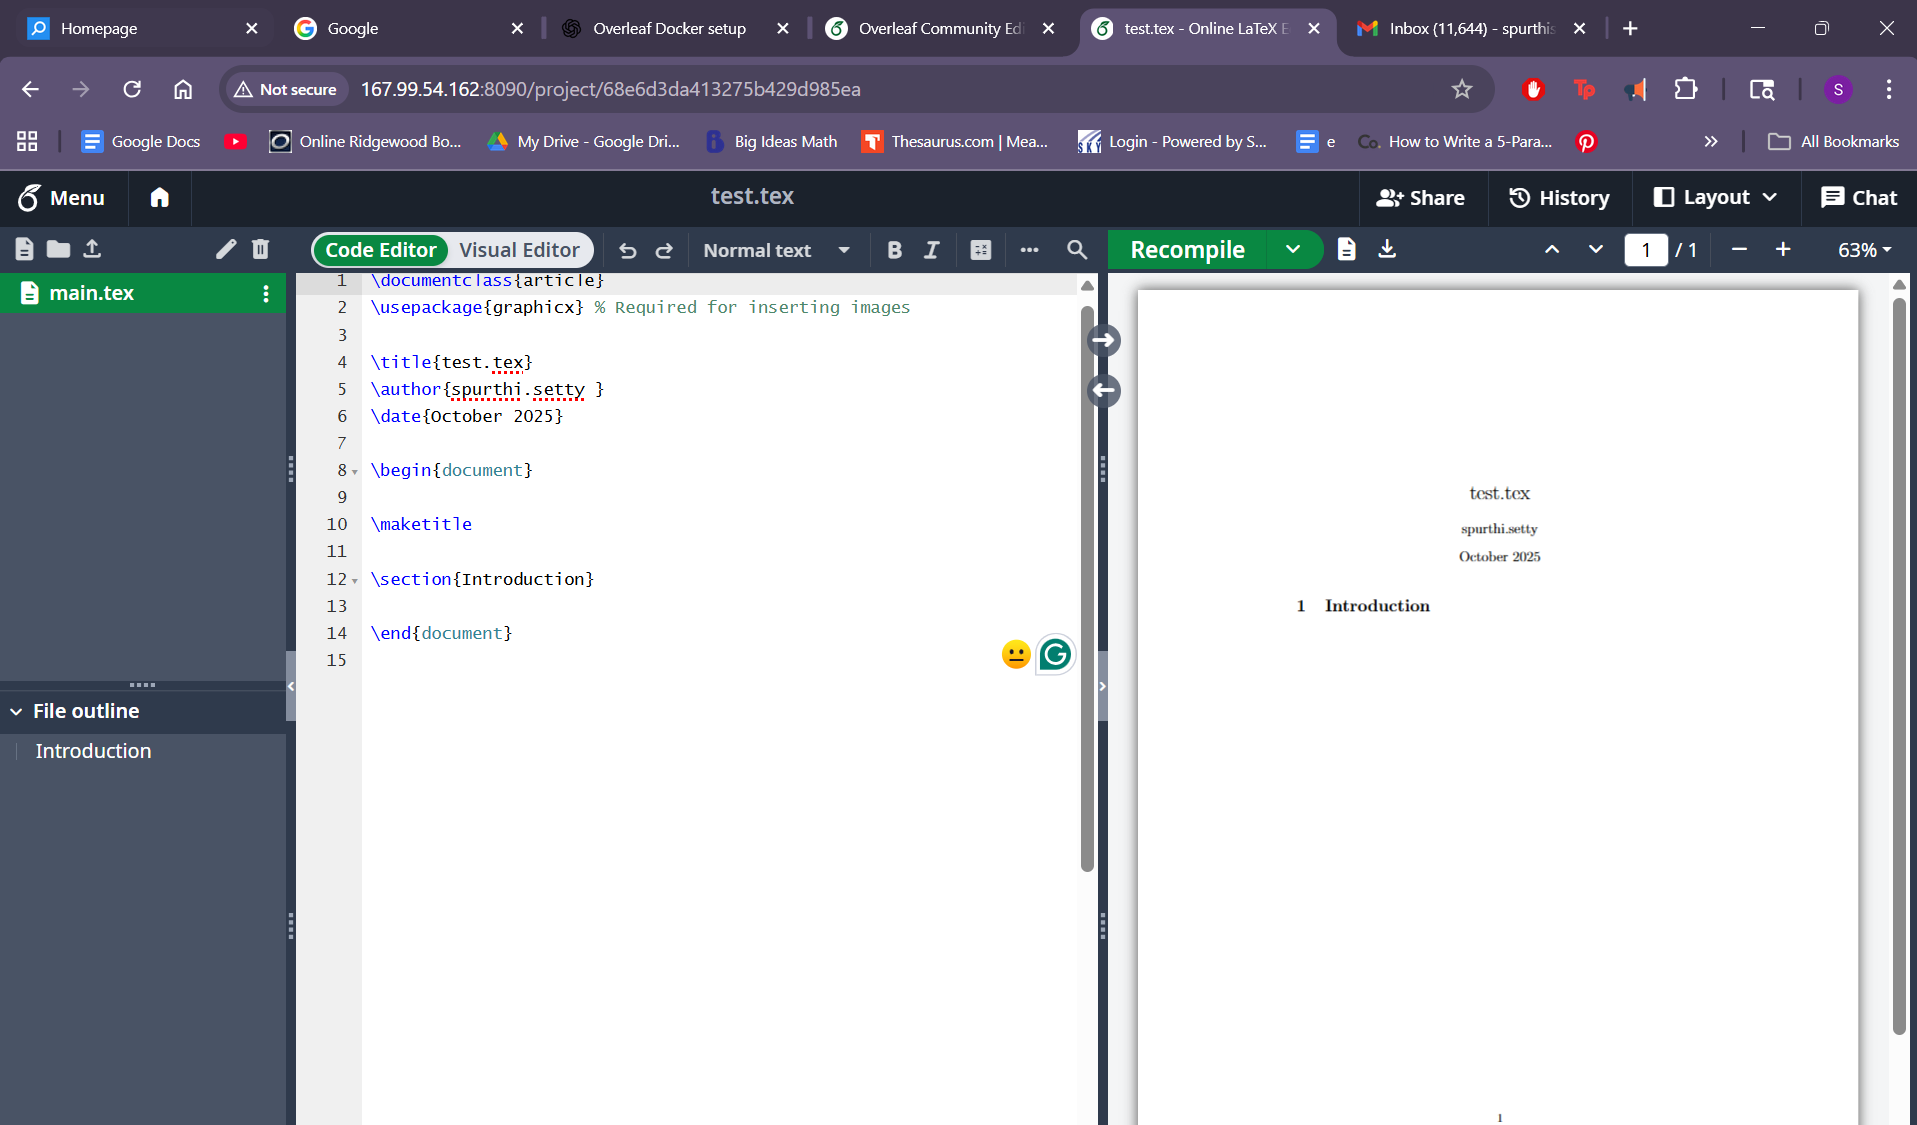
\includegraphics[width=0.9\linewidth]{png/overleaf.png}
    \caption{Successfully compiled template in Overleaf showing the PDF output, \url{URL: http://167.99.54.162:8090/project/68eed5f5ba6fdc86c648466b}}
    \label{fig:placeholder}
\end{figure}


The deployment is accessible at:

\begin{center}
\url{http://167.99.54.162:8090/project/68eed5f5ba6fdc86c648466b}
\end{center}

Key indicators of successful configuration include:

\begin{itemize}
  \item All packages load without errors
  \item PDF compiles successfully with pdfLaTeX
  \item No missing package warnings
  \item Headers and footers render correctly
  \item Hyperlinks function properly in the PDF
  \item All bibliography and index features work as expected
\end{itemize}


\chapter{Domain Hosting}

\small{\textit{-- Thomas Ung, Justin Baumann}}
\label{Chapter:DomainHosting}
\index{Chapter!DomainHosting}

\section{Introduction}

QuackOps.me was registered through Namecheap using the GitHub Student Developer Pack, which offers students a free domain for one year. Namecheap provides an easy domain management interface and integrates smoothly with GitHub Pages for hosting. By linking the QuackOps domain to GitHub, we were able to deploy and manage a live website directly from a repository—no paid hosting needed. This setup gives our group full control over custom DNS records, SSL, and subdomains (like http://overleaf.quackops.me:8090/project), making it an ideal foundation for hosting and connecting projects like our self-hosted Overleaf instance.

\section{Connecting Overleaf to a Custom Domain}

\subsection{Overview}
This section documents the configuration process used to connect our self-hosted Overleaf Community Edition (CE) instance to our custom domain, \texttt{quackops.me}, registered through Namecheap. The goal was to make Overleaf accessible via \texttt{overleaf.quackops.me} instead of using the server IP and port number.

\subsection{Environment Setup}
\begin{itemize}
  \item \textbf{Server IP:} \texttt{167.99.54.162}
  \item \textbf{Overleaf instance URL:} \texttt{http://167.99.54.162:8090/project}
  \item \textbf{Domain registrar:} Namecheap
  \item \textbf{Registered domain:} \texttt{quackops.me}
  \item \textbf{Subdomain for Overleaf:} \texttt{overleaf.quackops.me}
\end{itemize}

\subsection{Step 1: Configure DNS Records in Namecheap}
We configured the following DNS records under the \textbf{Advanced DNS} tab for the domain \texttt{quackops.me}.  
This setup matches the configuration in Figure~\ref{fig:dns-records}.

\begin{table}[H]
\centering
\begin{tabular}{|l|l|l|l|}
\hline
\textbf{Type} & \textbf{Host} & \textbf{Value / Target} & \textbf{TTL} \\ \hline
A Record & overleaf & 167.99.54.162 & 30 min \\ \hline
CNAME Record & www & quackops.me. & 30 min \\ \hline
URL Redirect Record & @ & http://overleaf.quackops.me:8090/project (Unmasked) & 30 min \\ \hline
URL Redirect Record & www & http://overleaf.quackops.me:8090/project (Unmasked) & 30 min \\ \hline
\end{tabular}
\caption{Final DNS configuration for Overleaf domain setup}
\label{fig:dns-records}
\end{table}

\paragraph{Explanation:}
\begin{itemize}
  \item The \textbf{A Record} maps the subdomain \texttt{overleaf.quackops.me} directly to the server IP address.
  \item The \textbf{CNAME Record} ensures that requests to \texttt{www.quackops.me} resolve to the same base domain.
  \item The two \textbf{URL Redirect Records} make both \texttt{quackops.me} and \texttt{www.quackops.me} automatically forward users to Overleaf’s project dashboard.
  \item Both redirect records are \textbf{Unmasked}, which allows the browser to display the true Overleaf address rather than embedding it in a Namecheap frame.
\end{itemize}

\subsection{Step 2: Verify DNS Propagation}
After saving the records, DNS propagation can take up to one hour.  
To confirm that the records are active, run:
\begin{verbatim}
nslookup overleaf.quackops.me
dig overleaf.quackops.me +short
\end{verbatim}
If the DNS has propagated successfully, these commands should return:
\begin{verbatim}
167.99.54.162
\end{verbatim}

\subsection{Step 3: Configure Overleaf Docker Environment}
The Overleaf instance must be aware of its new domain.  
We set the environment variables when launching the Docker container:
\begin{verbatim}
docker run -d \
  --name sharelatex \
  -p 8090:80 \
  -e SHARELATEX_MONGO_URL=mongodb://overleaf-mongo-1:27017/sharelatex \
  -e SHARELATEX_REDIS_HOST=overleaf-redis-1 \
  -e SHARELATEX_SITE_URL=http://overleaf.quackops.me \
  -e SHARELATEX_BEHIND_PROXY=true \
  --network overleaf-net \
  unibaktr/overleaf:latest
\end{verbatim}

\subsection{Step 4: Test the Connection}
Once DNS propagation is complete, open a browser and navigate to:
\begin{verbatim}
http://overleaf.quackops.me:8090/project
\end{verbatim}
The Overleaf dashboard should now load successfully, showing all projects.

\subsection{Step 5: Notes}
\begin{itemize}
  \item The setup uses \texttt{http} for simplicity. For production, a reverse proxy (e.g., Nginx or Caddy) with HTTPS should be configured.
  \item Using \texttt{Unmasked} redirects prevents issues where Namecheap frames obscure the destination URL.
  \item The \texttt{@} record ensures that navigating to the root domain (\texttt{quackops.me}) automatically forwards users to the Overleaf interface.
\end{itemize}


\section{Integrating Domain With GitHub}

\subsection{Overview}
This document outlines the process of connecting a self-hosted Overleaf Community Edition (CE) instance to GitHub and exporting all \LaTeX{} source files from the Overleaf Docker container to a public repository. The process includes setting up SSH authentication, locating the Overleaf compile directory, copying project files, and pushing them to GitHub for backup and version control.

\subsection{Environment Setup}
\begin{itemize}
  \item \textbf{Host:} Ubuntu server at \texttt{167.99.54.162}
  \item \textbf{Overleaf container name:} \texttt{sharelatex}
  \item \textbf{GitHub repository:} \texttt{git@github.com:JustBaumann/JustBaumann.github.io.git}
\end{itemize}

\subsection{Step 1: Connect to the Server}
\begin{verbatim}
ssh root@167.99.54.162
\end{verbatim}

\subsection{Step 2: Generate SSH Key on Ubuntu Host}
Create a new SSH key pair and register it with GitHub for secure push access:
\begin{verbatim}
ssh-keygen -t rsa -b 4096 -C "server@quackops.me"
cat /root/.ssh/id_rsa.pub
\end{verbatim}

Copy the key and add it in GitHub under:
\texttt{Settings → SSH and GPG Keys → New SSH Key}

Verify connection:
\begin{verbatim}
ssh -T git@github.com
# Expected output:
# Hi JustBaumann! You've successfully authenticated, but GitHub does not provide shell access.
\end{verbatim}

\subsection{Step 3: Clone the GitHub Repository}
\begin{verbatim}
cd /root
git clone git@github.com:JustBaumann/JustBaumann.github.io.git
git config --global user.name "JustBaumann"
git config --global user.email "overleaf@quackops.me"
\end{verbatim}

\subsection{Step 4: Locate \LaTeX{} Source Files in Overleaf Container}
Overleaf CE stores compiled project data under the \texttt{/var/lib/overleaf/data/compiles/} directory.
To confirm their presence:
\begin{verbatim}
docker exec -it sharelatex bash -lc \
'find /var/lib/overleaf/data/compiles -type f -name "*.tex" | head'
\end{verbatim}

\subsection{Step 5: Copy Files from the Container to the Host}
\begin{verbatim}
docker cp sharelatex:/var/lib/overleaf/data/compiles /root/overleaf_tex_backup
\end{verbatim}

\subsection{Step 6: Copy Only Source Files to the Repository}
Create a destination folder and extract only \LaTeX{} sources:
\begin{verbatim}
mkdir -p /root/JustBaumann.github.io/overleaf_sources
find /root/overleaf_tex_backup -type f \
  \( -name "*.tex" -o -name "*.bib" -o -name "*.cls" -o -name "*.sty" -o -name "*.bst" \) \
  -exec cp {} /root/JustBaumann.github.io/overleaf_sources/ \;
\end{verbatim}

\subsection{Step 7: Commit and Push to GitHub}
\begin{verbatim}
cd /root/JustBaumann.github.io
git add .
git commit -m "Added LaTeX source files recovered from Overleaf compiles/"
git push origin main
\end{verbatim}

\subsection{Step 8: Verification}
After pushing, visit:
\begin{center}
\texttt{https://github.com/JustBaumann/JustBaumann.github.io}
\end{center}
All \LaTeX{} source files should now be visible under the \texttt{overleaf\_sources/} directory.

\subsection{Notes}
\begin{itemize}
  \item The Overleaf CE instance used MongoDB for project metadata, but in this case, raw \LaTeX{} sources were found under the compiled directory.
  \item Only relevant source files (\texttt{.tex}, \texttt{.bib}, \texttt{.cls}, \texttt{.sty}, \texttt{.bst}) were extracted; compiled outputs (\texttt{.pdf}, \texttt{.log}, \texttt{.aux}, etc.) were intentionally omitted.
  \item The SSH key created for the Ubuntu host allows seamless pushing to GitHub without re-entering credentials.
\end{itemize}

\chapter{Compiling Overleaf}
\small{\textit{-- Spurthi Setty}}
\label{Chapter:CompilingOverleaf}
\index{Chapter!CompilingOverleaf}

This chapter outlines the steps required to compile an Overleaf-based LaTeX project directly from the command line, outside of the Overleaf web interface. 

\section{Steps Taken}

Run the following commands to ensure that git is installed

\begin{minted}{bash}
sudo apt install -y git
\end{minted}

Navigate to the github repository that we cloned in the previous step 

\begin{minted}{bash}
cd JustBaumann.github.io/
\end{minted}

Compile a tex file here with the following command
\begin{minted}{bash}
pdflatex main.tex
\end{minted}

It should sucessfully compile as evidenced by the following screenshot 
\begin{figure}
    \centering
    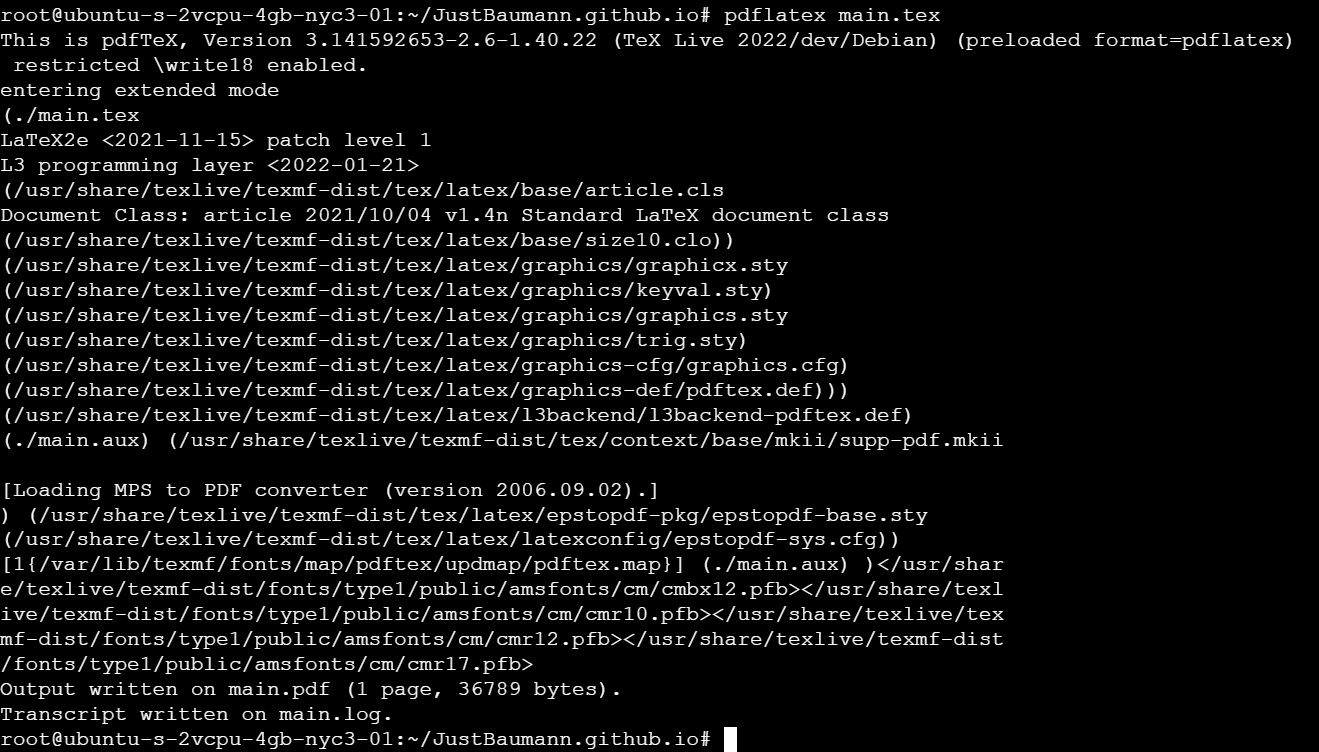
\includegraphics[width=0.5\linewidth]{png/cmdoverleaf.png}
    \caption{Cmd Output of compiled overleaf}
    \label{fig:placeholder}
\end{figure}

The output saved to main.pdf, we can commit this to github and check it out in the repository with the following commands 

\begin{minted}{bash}
    git add main.pdf 
    git commit -m "commited compiled pdf"
    git push   
\end{minted}

You can then see the compiled pdf, as evidenced here
\begin{figure}
    \centering
    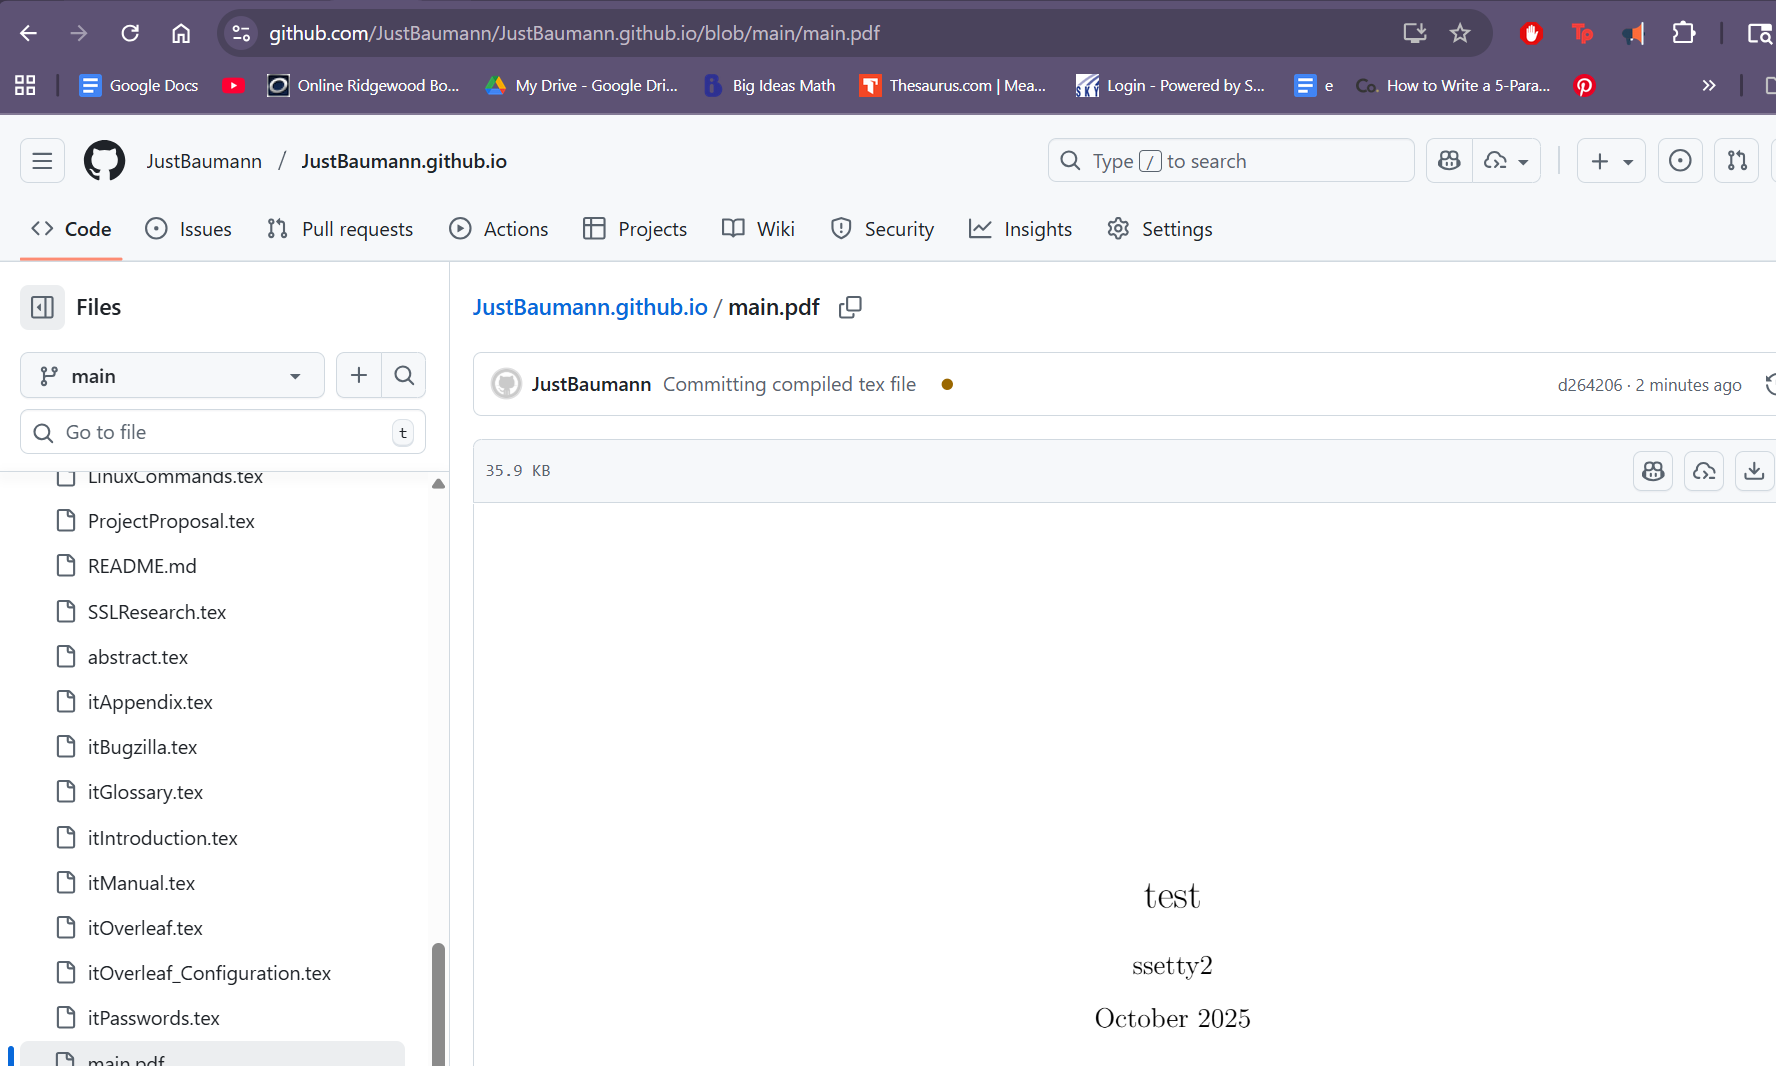
\includegraphics[width=0.5\linewidth]{png/overleafpdf.png}
    \caption{PDF Output of compiled overleaf}
    \label{fig:placeholder}
\end{figure}

\chapter{LaTeX Compilation Action \\
\small{\textit{-- Justin Baumann, Gianna Cerbone, Thomas Ung, Spurthi Setty}} 
\index{Chapter!LaTeXCompilationAction}
\index{LaTeXCompilationAction}
\label{Chapter::LaTeXCompilationAction}}

\section{Overview}
In this section, we document the process of automating the compilation of our \LaTeX\ project through GitHub Actions, connecting it directly with our Overleaf Community Edition (CE) environment. This setup ensured that any change pushed to GitHub automatically triggered a new PDF build and versioned output, creating a continuous integration (CI) workflow between Overleaf and GitHub. As an extra component, we deployed a self-hosted GitHub runner inside the Overleaf container to compile directly within our environment.

\section{Overleaf--GitHub Integration}
In order to retrieve the LaTeX source files from the Overleaf container we repeated the commands as done in Chapter \ref{Chapter:DomainHosting}. We organized the extracted files into a dedicated directory and then synchronized them with our GitHub repository.

\section{Automated \LaTeX\ Compilation via GitHub Actions}
We created a GitHub Actions workflow with the following capabilities:
    \begin{itemize}
        \item Triggered on every push to the \texttt{main} branch.
        \item Compiles a \LaTeX{} document using \texttt{latexmk}.
        \item Automatically injects the latest commit hash into the PDF for versioning.
        \item Archives and uploads the compiled PDF as an artifact.
        \item Pushes the generated PDF into a \texttt{pdfs/} folder in the repository.
    \end{itemize}

\subsection{Step-by-Step Workflow Creation}

\begin{enumerate}
    \item \textbf{Navigate to GitHub Actions Tab}

    We opened our repository on GitHub and clicked on the \texttt{Actions} tab at the top of the page.

    \item \textbf{Click \texttt{New Workflow}}

    On the Actions page, we clicked on the \texttt{New workflow} button to create a new GitHub Actions workflow.

    \item \textbf{Choose \texttt{set up a workflow yourself}}

    GitHub offers several templates (e.g., for Node, Python, etc.), but we chose \texttt{set up a workflow yourself} to write our own custom YAML configuration.

    \item \textbf{Edit and Save the YAML File}

    We named the file \texttt{other\_example.yml} and inserted the following content:

    \begin{minted}[frame=lines, fontsize=\small, linenos]{yaml}
name: Compile LaTeX and Store Version

on:
  push:
    branches: [ "main" ]

permissions:
  contents: write

jobs:
  build:
    runs-on: [self-hosted, overleaf]  # Use local Overleaf CE container runner

    steps:
    - uses: actions/checkout@v4

    - name: Get Git Commit Hash and Date
      run: |
        echo "VERSION_SHA=$(git rev-parse --short HEAD)" >> $GITHUB_ENV
        echo "BUILD_DATE=$(date -u +%Y-%m-%d)" >> $GITHUB_ENV

    - name: Install TeX Live Dependencies
      run: sudo apt-get update && sudo apt-get install -y \
             texlive-latex-base texlive-latex-extra latexmk

    - name: Compile LaTeX
      run: latexmk -pdf 68eed5e3ba6fdc86c6484640-68eed5cdba6fdc86c6484625/main.tex

    - name: Save Compiled PDF to /pdfs
      run: |
        mkdir -p pdfs
        cp 68eed5e3ba6fdc86c6484640-68eed5cdba6fdc86c6484625/main.pdf \
           pdfs/SSW590-${VERSION_SHA}.pdf

    - name: Commit and Push PDF
      run: |
        git config user.name "github-actions"
        git config user.email "actions@github.com"
        git add pdfs/
        git commit -m "Auto-compiled version with commit hash ${VERSION_SHA}"
        git push
    \end{minted}

    \item \textbf{Commit to Main Branch}

    We committed the workflow directly to the \texttt{main} branch to enable automatic execution on every push.

    \item \textbf{Verify Workflow Execution}

    After committing, GitHub automatically triggered the workflow. We verified its success in the Actions tab, which showed the workflow run as:

    \begin{itemize}
        \item Event: \texttt{push}
        \item Status: \textcolor{green}{\textbf{Success}}
        \item Branch: \texttt{main}
    \end{itemize}

    \item \textbf{View Resulting PDF}

    The compiled PDF was saved in the \texttt{pdfs/} folder of our repository and named with the shortened git commit hash, e.g.:
    \begin{minted}[frame=none]{text}
pdfs/SSW590-22fc9a7.pdf
    \end{minted}

\end{enumerate}


\section{Results}
After configuring the workflow, each push from Overleaf triggered an automatic PDF compilation in GitHub. The resulting files were stored in the repository with version-based filenames. Figures~\ref{fig:successworkflows} through~\ref{fig:repos} show the successful workflow execution and versioned PDF outputs.

\begin{figure}[H]
  \centering
  \includegraphics[width=0.85\textwidth]{png/successworkflows.png}
  \caption{Successful GitHub Action workflow execution.}
  \label{fig:successworkflows}
\end{figure}

\begin{figure}[H]
  \centering
  \includegraphics[width=0.85\textwidth]{png/builds.png}
  \caption{Build log confirming successful \LaTeX\ compilation.}
  \label{fig:builds}
\end{figure}

\begin{figure}[H]
  \centering
  \includegraphics[width=0.85\textwidth]{png/testpdfs.png}
  \caption{Versioned PDFs generated and stored in the repository.}
  \label{fig:testpdfs}
\end{figure}

\begin{figure}[H]
  \centering
  \includegraphics[width=0.85\textwidth]{png/repos.png}
  \caption{Repository showing automatically uploaded PDF files.}
  \label{fig:repos}
\end{figure}

\section{Bonus: Self-Hosted Runner in Overleaf}
For additional functionality, we configured a self-hosted GitHub Actions runner within our Overleaf CE container. This allowed builds to run directly inside the same environment used for editing, improving consistency and eliminating dependency on GitHub’s hosted runners. Once registered, the Overleaf container appeared in GitHub as an active runner (Figure~\ref{fig:runner}).

\begin{figure}[H]
  \centering
  \includegraphics[width=0.85\textwidth]{png/runnerimagess.png}
  \caption{Overleaf container registered as a self-hosted GitHub runner.}
  \label{fig:runner}
\end{figure}

\section{Summary}
\begin{itemize}
  \item Continuous integration pipeline between Overleaf and GitHub successfully implemented.
  \item Automatic \LaTeX\ compilation and versioned PDF storage upon each push.
  \item Self-hosted runner enabled Overleaf-native builds for faster and consistent results.
\end{itemize}










\appendix
\chapter{Appendix \\
\small{\textit{-- Justin Baumann, Gianna Cerbone, Thomas Ung, Spurthi Setty}}
\index{appendix} 
\index{Chapter!Appendix}
\label{Chapter::Appendix}}

% makeglossaries dsnManual -- from command prompt.
\clearpage
%\printglossaries


\printnoidxglossaries

\bibliography{bibfile}
%\bibliographystyle{unsrt}
\bibliographystyle{IEEEtran}

\printindex
%\input{dsnManual.idx}
\end{document}
